%% Lab Report for EEET2493_labreport_template.tex
%% V1.0
%% 2019/01/16
%% This is the template for a Lab report following an IEEE paper. Modified by Francisco Tovar after Michael Sheel original document.


%% This is a skeleton file demonstrating the use of IEEEtran.cls
%% (requires IEEEtran.cls version 1.8b or later) with an IEEE
%% journal paper.
%%
%% Support sites:
%% http://www.michaelshell.org/tex/ieeetran/
%% http://www.ctan.org/pkg/ieeetran
%% and
%% http://www.ieee.org/

%%*************************************************************************
%% Legal Notice:
%% This code is offered as-is without any warranty either expressed or
%% implied; without even the implied warranty of MERCHANTABILITY or
%% FITNESS FOR A PARTICULAR PURPOSE! 
%% User assumes all risk.
%% In no event shall the IEEE or any contributor to this code be liable for
%% any damages or losses, including, but not limited to, incidental,
%% consequential, or any other damages, resulting from the use or misuse
%% of any information contained here.
%%
%% All comments are the opinions of their respective authors and are not
%% necessarily endorsed by the IEEE.
%%
%% This work is distributed under the LaTeX Project Public License (LPPL)
%% ( http://www.latex-project.org/ ) version 1.3, and may be freely used,
%% distributed and modified. A copy of the LPPL, version 1.3, is included
%% in the base LaTeX documentation of all distributions of LaTeX released
%% 2003/12/01 or later.
%% Retain all contribution notices and credits.
%% ** Modified files should be clearly indicated as such, including  **
%% ** renaming them and changing author support contact information. **
%%*************************************************************************


\listfiles
\documentclass[review]{elsarticle}

\usepackage{lineno,hyperref}
\modulolinenumbers[5]

\journal{Journal of \LaTeX\ Templates}

% *** CITATION PACKAGES ***

\usepackage[style=ieee]{biblatex} 
\bibliography{example_bib.bib}    %your file created using JabRef

\usepackage{dirtytalk}

\usepackage{nomencl}
\makenomenclature

\renewcommand{\nomname}{List of Symbols}
%\renewcommand{\nompreamble}{The next list describes several symbols that will be later used within the body of the document}

\usepackage{amssymb}

\usepackage{etoolbox}
\renewcommand\nomgroup[1]{%
  \item[\bfseries
  \ifstrequal{#1}{A}{Railway network}{%
  \ifstrequal{#1}{B}{Power network}{%
  \ifstrequal{#1}{C}{Interdependency}{%
  \ifstrequal{#1}{D}{Initiating event}{%
  \ifstrequal{#1}{E}{Cascading failures}{%
  \ifstrequal{#1}{F}{Vulnerability analysis}{%
  \ifstrequal{#1}{G}{Simulation}{}}}}}}}%
]}

% *** MATH PACKAGES ***
\usepackage{amsmath}
\usepackage{mathtools}
\DeclarePairedDelimiter\ceil{\lceil}{\rceil}
\DeclarePairedDelimiter\floor{\lfloor}{\rfloor}

\usepackage{algorithm}
\usepackage{algpseudocode}

\usepackage{amssymb}

% *** PDF, URL AND HYPERLINK PACKAGES ***
\usepackage{url}
% correct bad hyphenation here
\hyphenation{op-tical net-works semi-conduc-tor}
\usepackage{graphicx}  %needed to include png, eps figures
\usepackage{float}  % used to fix location of images i.e.\begin{figure}[H]

\begin{document}


\begin{frontmatter}

\title{A modeling framework for vulnerability analysis of interdependent railway and power networks}
%\tnotetext[mytitlenote]{Fully documented templates are available in the elsarticle package on %\href{http://www.ctan.org/tex-archive/macros/latex/contrib/elsarticle}{CTAN}.}

%% Group authors per affiliation:
\author{Andrea Bellè\corref{mycorrespondingauthor}}
\cortext[mycorrespondingauthor]{Corresponding author}
\ead{andrea.belle@centralesupelec.fr}
\author{Zhiguo Zeng, Anne Barros}
\address{Chair on Risk and Resilience of Complex Systems, Laboratoire Génie Industriel, CentraleSupélec, Université Paris-Saclay}
%\fntext[myfootnote]{Since 1880.}

%% or include affiliations in footnotes:
%\author[mymainaddress,mysecondaryaddress]{Elsevier Inc}
%\ead[url]{www.elsevier.com}




%\address[mymainaddress]{1600 John F Kennedy Boulevard, Philadelphia}
%\address[mysecondaryaddress]{360 Park Avenue South, New York}

\begin{abstract}
Railway and power networks are among the most important critical infrastructures, and their vulnerability under different types of disrupting events has been extensively analyzed. However, the increasing degree of interconnection and interdependency between the two critical infrastructures makes it necessary to consider the multiple interdependencies when conducting vulnerability assessments. In this work, we focus on a railway network which depends on an external power network for the electricity supply. Firstly, we propose a modeling framework for an interdependent railway-power network which accounts for cascading failures within and between networks. Secondly, the framework is used to analyze how the interdependencies affect the vulnerability of the railway network considering different random and localized failure patterns in the power network. Thirdly, we evaluate how the vulnerability of the railway and the power network is affected by simultaneous failures in both the networks. With the proposed model, we show that failures in the power network have a considerable negative impact on the railway network. On the contrary, our analysis shows that failures in the railway network surprisingly reduce the vulnerability of the power network. In addition, in the case of simultaneous failures, we highlight the importance of considering the interdependencies on the precise estimate of the negative consequences in both the two individual networks.
\end{abstract}

\begin{keyword}
Critical infrastructures, vulnerability, interdependent networks, cascading failures, power, railway
\end{keyword}

\end{frontmatter}

\linenumbers

\mbox{}



  \nomenclature[A]{$\mathbf{G_r}$}{Graph representing the railway network }
  \nomenclature[A]{$\mathbf{V_r}$}{Set of nodes in railway network }
  \nomenclature[A]{$v_{r,i}$ }{ Node $i$ in the railway network, representing station $i$ }
  \nomenclature[A]{$N_r$ }{ Number of nodes in railway network}
  \nomenclature[A]{$\mathbf{E_r}$ }{ Set of edges in railway network }
  \nomenclature[A]{$e_{r,i}$ }{ Edge $i$ in railway network, representing railway $i$ }
  \nomenclature[A]{$M_r$ }{ Number of edges in railway network}
  \nomenclature[A]{$\mathbf{C_r}$ }{Set of components in railway network}

  
  \nomenclature[B]{$\mathbf{G_p}$}{ Graph representing the power network }
  \nomenclature[B]{$\mathbf{V_p}$ }{ Set of nodes in power network }
  \nomenclature[B]{$v_{p,i}$ }{ Node $i$ in the power network, representing electrical bus $i$ }
  \nomenclature[B]{$N_p$ }{ Number of nodes in power network}
  \nomenclature[B]{$\mathbf{E_p}$ }{ Set of edges in power network }
  \nomenclature[B]{$e_{p,i}$ }{ Edge $i$ in power network, representing transmission line $i$ }
  \nomenclature[B]{$M_p$ }{Number of edges in power network}
  \nomenclature[B]{$\mathbf{C_p}$ }{ Set of components in power network}
  \nomenclature[B]{$\mathbf{N_G}$}{Set of generators in power network  }
  \nomenclature[B]{$N_G$}{Number of generators in power network  }
  \nomenclature[B]{$G_i$ }{ Generator $i$ in power network }
  \nomenclature[B]{$\mathbf{N_L}$}{Set of loads in power network }
  \nomenclature[B]{$N_L$}{Number of loads in power network  }
  \nomenclature[B]{$L_i$ }{ Load $i$ in power network }
  
  \nomenclature[C]{$\mathbf{E_{r \leftarrow p}}$ }{ Set of interdependency edges between railway and power network }
  \nomenclature[C]{$e_{r,p}^{i \leftarrow j,k}$ }{ Interdependency edge between station $i$ and electrical bus $j$ with load $k$ }
  
  \nomenclature[D]{$\mathbf{V_{p,i}^{reg}}$ }{ Set of nodes in region $i$ of power network }
  \nomenclature[D]{$v_{p,i,j}^{reg}$ }{ Node $j$ in region $i$ of power network}
  \nomenclature[D]{$N_{p,i}^{reg}$ }{ Number of nodes in region $i$ of power network}
  \nomenclature[D]{$\mathbf{E_{p,i}^{reg}}$ }{ Set of edges in region $i$ of power network }
  \nomenclature[D]{$e_{p,i,j}^{reg}$ }{ Edge $j$ in region $i$ of power network}
  \nomenclature[D]{$M_{p,i}^{reg}$ }{ Number of edges in region $i$ of power network}
  \nomenclature[D]{$\mathbf{C_{p,i}^{reg}}$ }{ Set of components in region $i$ of power network}
  \nomenclature[D]{$\mathbf{V_{r,i}^{reg}}$ }{ Set of nodes in region $i$ of railway network }
  \nomenclature[D]{$v_{r,i,j}^{reg}$ }{ Node $j$ in region $i$ of railway network}
  \nomenclature[D]{$N_{r,i}^{reg}$ }{ Number of nodes in region $i$ of railway network}
  \nomenclature[D]{$\mathbf{E_{r,i}^{reg}}$ }{ Set of edges in region $i$ of railway network }
  \nomenclature[D]{$e_{r,i,j}^{reg}$ }{ Edge $j$ in region $i$ of railway network}
  \nomenclature[D]{$M_{r,i}^{reg}$ }{ Number of edges in region $i$ of railway network}
  \nomenclature[D]{$\mathbf{C_{r,i}^{reg}}$ }{ Set of components in region $i$ of railway network}
  \nomenclature[D]{$\mathbf{N_f}$ }{ Set of components to remove in the initiating event }
  \nomenclature[D]{$n_{f,i}$ }{ Component $i$ to remove in the initiating event }
  \nomenclature[D]{$N_{fail}$ }{ Number of elements to remove in the initiating event }
  \nomenclature[D]{$f$ }{ Fraction of components to remove in the initiating event}
  \nomenclature[D]{$p_{ie}$ }{ Probability of being selected for a removal for each component}
  
  \nomenclature[E]{$\mathbf{N^r_{s,i}}$ }{ Set of stations directly connected with a railway to station $i$}
  \nomenclature[E]{$\mathbf{N^r_{rw,i}}$ }{ Set of stations connected by railway $i$} 
  \nomenclature[E]{$S^r_{s,i}$ }{ Binary functional state of station $i$}
  \nomenclature[E]{$S^r_{rw,i}$ }{ Binary functional state of railway $i$} 
  \nomenclature[E]{$S^p_{l,i}$ }{ Binary functional state of transmission line $i$}
  \nomenclature[E]{$\mathbf{P_G}$ }{ Set of nominal generator power}
  \nomenclature[E]{$\mathbf{P_L}$ }{ Set of nominal load power}
  \nomenclature[E]{$P_{G,i}$ }{ Nominal power of generator $i$}
  \nomenclature[E]{$P_{L,i}$ }{ Nominal power of load $i$}
  \nomenclature[E]{$P_{G,i}^{max}$ }{ Maximum power of generator $i$}
  \nomenclature[E]{$P_{L,i}^{max}$ }{ Maximum power of load $i$}
  \nomenclature[E]{$\mathbf{F_l}$ }{ Set of line power flows}
  \nomenclature[E]{$F_{l,i}$ }{ Power flow at line $i$} 
  \nomenclature[E]{$F_{l,i}^{max}$ }{ Power flow capacity at line $i$} 
  \nomenclature[E]{$W$ }{ Load penalty constant} 
  \nomenclature[E]{$\mathbf{G'}$}{ Graph after a disruptive event }
  \nomenclature[E]{$\mathbf{V'}$ }{ Set of nodes after a disruptive event}
  \nomenclature[E]{$\mathbf{E'}$ }{ Set of edges after a disruptive event }
  \nomenclature[E]{$\mathbf{P_G}'$ }{ Set of nominal generator power after a disruptive event}
  \nomenclature[E]{$\mathbf{P_L}'$ }{ Set of nominal load power after a disruptive event}
  \nomenclature[E]{$S^p_{l,k}$ }{ Binary functional state of line $k$}   
  \nomenclature[E]{$R_{P_L,k}$ }{ Load shedding ratio of load $k$}    
  \nomenclature[E]{$\mathbf{R_{P_L}}'$ }{ Set of load shedding ratios} 
  \nomenclature[E]{$T_{r \leftarrow p}^{P_L} $ }{ Tolerance threshold for station load shedding} 


  \nomenclature[F]{$V$ }{ Vulnerability index}
  \nomenclature[F]{$PI$ }{ performance indicator}
  \nomenclature[F]{$A_r$ }{ Accessibility of railway network}   
  \nomenclature[F]{$n_a^i$ }{ Number of stations accessible from station $i$}    
  \nomenclature[F]{$FDNS$ }{ Fraction of Demand Not Supplied} 

  \nomenclature[G]{$\Bar{V}$ }{ Average vulnerability index}
  \nomenclature[G]{$CI_{95}$ }{ $95\%$ confidence intervals}
  \nomenclature[G]{$Z$ }{ Confidence intervals constant}   
  \nomenclature[G]{$\sigma$ }{ Standard deviation estimation}    
  \nomenclature[G]{$N_{exp}$ }{ Number of Monte Carlo simulations}

\printnomenclature



	\section{Introduction}
	\subsection{Motivation}
	Critical infrastructures, such as transportation, healthcare, energy systems, water supply systems and telecommunication networks, are large-scale systems which provides essential goods and services for the society. Their malfunctioning and failure can heavily affect the safety and the socio-economic stability of a population. Developing highly reliable infrastructures is, thus, an important issue. Lately, due to the increasing degree of interconnection and interdependency, infrastructures has transformed from isolated individual systems to a highly interconnected system-of-systems. This evolution, despite leading to improvements of performance, has introduced also new failure modes and threats \cite{buldyrev2010catastrophic}. Critical infrastructures are often analyzed in terms of their vulnerability to different types and magnitudes of disrupting events. Vulnerability analysis is defined in \cite{johansson2011vulnerability} as the process of \say{systematic  and  comprehensive  identifying the  possible  states  a  system  can  be  put  into,  due  to  specific  strains,  and  estimating the negative consequences associated with them}. This analysis has proved to be useful in design and prevention stages, as it gives an overview of how a system responds to different disruptive situations.
	
	Transportation systems, and in particular railway networks, are acknowledged as one of the most important infrastructures. It is recognized that railway systems are dependent on several internal and external subsystems and infrastructures \cite{pant2016vulnerability}. The dependency on external power systems is of particular relevance, as the latter supply the electricity necessary for the functioning of the systems and equipment of the railway network. In case of a disruptive event in a power grid, this strong dependency can lead to considerable negative consequences on the railway system. In fact, power outages and blackouts have long been observed as important causes of railway networks disruption, as what happened in Great Britain during August 2019 \cite{GBblackout_1}\cite{GBblackout_2}. Given this strong dependency, it is important to raise the awareness of power network-induced risks in railway networks \cite{uicenews616}.\\
	In the literature are limited to approaches where the cascading failures in power networks are not considered or modeled with a simplified approach based on complex network theory. These frameworks recognize the importance of the power systems for the railway networks functionality, but without modeling and analyzing in details the effect of cascading failures in power networks and their repercussions on railway networks. With this work, we aim to complement the available literature with a modeling framework for interdependent railway and power networks which accounts for flow-based characterization of cascading failures in power networks and their consequences in railway networks.
	
	\subsection{Related work}
	Railway systems have been intensively analyzed in the context of vulnerability analysis. Several works are available in literature, addressing different disruptive events and analyzing the negative consequences with various indicators (e.g. topological disruption, loss of passengers and/or rolling stocks, delays, etc.). In \cite{mattsson2015vulnerability} and \cite{reggiani2015transport}, the authors discuss the concepts of vulnerability and resilience in transportation networks from a research perspective, including also a comprehensive literature review. In \cite{ouyang2014comparisons}, the authors compare the vulnerability of the Chinese railway system using network-based and flow-based performance indicators. In \cite{chen2007network}, the vulnerability of a railway network is assessed in terms of accessibility and equilibrium flows. In \cite{ouyang2015vulnerability}, the authors perform a vulnerability analysis of complementary transportation networks, addressing the positive effect of interdependencies between complementary systems. In \cite{hong2015vulnerability}, the authors perform a vulnerability analysis of the Chinese railway system focusing on historical flooding data. In \cite{zhang2016structural}, an analysis of the vulnerability of different high-speed railway networks using network-based metrics is performed. In \cite{yan2017pre}, an investment optimization framework for minimizing loss of service in a railway network during earthquake scenarios is proposed. In \cite{ye2019assessing}, the vulnerability analysis of a railway network considering partial failures of nodes is presented. In \cite{lu2019vulnerability}, the vulnerability analysis of a urban railway network taking into account multi-modal public transport network is proposed. In \cite{hong2019spatiotemporal}, the authors analyze the vulnerability of railway systems including  spatio-temporal features. In \cite{fang2020vulnerability}, the vulnerability analysis of the Chinese high-speed railway network under random and spatially localized failures is performed. In \cite{berche2009resilience} and \cite{berche2012transportation}, the public transportation systems of several cities are represented using network theory and their vulnerability under different types of random and targeted attacks is evaluated. In \cite{derrible2010complexity}, the topologies of several real metro networks and their implications in terms of robustness is evaluated using network theory. In \cite{rodriguez2014measuring}, the criticality and the vulnerability of the Madrid metro system is assessed. In \cite{de2012evaluating}, a passenger-based robustness analysis for transportation network is proposed, using the Barcelona metro system as a case-study. In \cite{gedik2014vulnerability}, the impact of disruptions in a supply chain based on a railroad transportation network is modeled and assessed.
	
	Since most modern railways are electrified, power systems have great potentials of causing extensive disruption in railway networks. Altough the vulnerability of the electrical networks has been relatively well-studied (see \cite{abedi2019review} and its references), only a few existing works discussed the vulnerability of interdependent railway and electrical networks. In \cite{zhang2014approach}, the authors propose a network-based approach for modeling the vulnerability analysis of a network-of-networks using as an example interdependent transportation, power and telecommunications, and including a network-based cascading failures model for the power network. A similar approach, also including a network-based cascading failures model for the power network, is proposed in \cite{zio2010modeling} and in \cite{zio2011modeling}, where the authors consider a fictitious railway network based on the topology of the Italian high-voltage grid, connected to the power and telecommunications networks, and they analyze its vulnerability taking into account safety margins and uncertainties. In \cite{johansson2010approach}, a modeling framework for the vulnerability analysis of a railway system dependent on electrical and telecommunications networks is proposed, including critical components and locations analysis. A similar approach is also proposed in \cite{johansson2011vulnerability}, where the dependence of the railway network on the external power grid is addressed but without considering the possibility of having cascading failures in the power grid. In \cite{pant2016vulnerability}, a mathematical framework for modeling the vulnerability analysis of a railway network considering its subsystems is presented; this study accounts for the dependency between the electricity and transportation, but without considering the external power grid. In \cite{adjetey2016model} and \cite{dorbritz2011assessing}, the resilience of railway networks is studied, also accounting for the dependency on the power subsystems.
	
	A common drawback of the existing researches on interdependent railway and electrical networks is that, cascading failures are not well considered in most of the works. Among the few works that considered cascading failure, only cascading failures within the power networks are considered \cite{zhang2014approach}, \cite{zio2010modeling}  \cite{zio2011modeling}. Furthermore, in these works, the cascading failures are modeled using an approach based on network theory \cite{motter2002cascade}\cite{crucitti2004model}, which is not capable to capture the realistic behaviors associated with the actual electrical power flows. It is clear that interdependent railway and power networks deserves a more detailed analysis, with a focus on a more realistic consideration of the cascading failures, in order to shed some light on the mutual risks of these interconnected systems.

	\subsection{Contribution}
	In this work, we propose a modeling framework for the vulnerability analysis of interdependent railway and power systems, which includes the evaluation of cascading failures within and between networks. For the power network, cascading failures are simulated with a dynamic model which accounts for the electrical flow within the elements. This feature allows for a more realistic characterization of cascading failures than network-based models, and it allows a better understanding of the effect of power outages on the railway network. With the proposed model, we confirm the high disruptive potential of the power network towards the railway network. We assess the importance of cascading failures in the power network in terms of magnitude and location of disruption in the railway. In addition, we also show that, when a disruptive event cause simultaneous failures in both the networks, it is important to evaluate the vulnerability of the single networks accounting for the interdependencies, in order to avoid an underestimation or overestimation of the negative consequences. The rest of this work is structured as follows: in section II, the main modeling frameworks are presented; in section III, the case-study utilized in this work is described; in section IV the results are presented; in section V the results and their implications are discussed and commented; in section VI, final remarks and possible developments are given.

	
	\section{Modeling framework}
	In this section, the main modeling approaches and assumptions are described. Each subsection describes a particular feature of the model: 
	\begin{itemize}
	    \item Network-based model: the railway and power systems topological features are described using network theory.
	    \item Modeling initiating events: the initial failures are simulated as removals of elements from the network.
	    \item Modeling cascading failures: removals of elements from a network can trigger a failure propagation within and between networks.
	    \item Modeling vulnerability: after the initiating event and the eventual propagation, the loss of performance in respect to the starting conditions is computed.
	\end{itemize}
	

	
	
	\subsection{Network-based model for interdependent railway and power systems}
	
	Network science is often used to describe the topology of both railway and power networks, thanks to its capacity to describe complex topologies and interactions with simple mathematical artifacts such as nodes and edges. A network is defined by a graph $\mathbf{G}=(\mathbf{V}, \mathbf{E})$, with $\mathbf{V} = \{ v_1, v_2,...,v_N \}$ representing the set of $N$ nodes (or vertices) and $\mathbf{E} = \{ e_1, e_2,...,e_M \}$ the set of $M$ edges. Each edge $k$ is also defined by a tuple $e_k=(v_i,v_j)$, which indicates the two nodes $v_i$ and $v_j$ connected by edge $k$.
	
	In a railway network $\mathbf{G_r}$, each node represents a station and each edge represents a railway track. The network is composed by a set of $N_r$ nodes $\mathbf{V_r}=\{ v_{r,1}, v_{r,2},...,v_{r,N_r} \}$ and a set of $M_r$ edges $\mathbf{E_r}=\{ e_{r,1}, e_{r,2},...,e_{r,M_r} \}$. Each edge $k$ connects two different nodes $v_{r,i}$ and $v_{r,j}$, as defined in the tuple $e_{r,k} = (v_{r,i}, v_{r,j})$.
	
	In the power network $\mathbf{G_p}$, nodes represent electrical buses and edges represent transmission lines. The network is composed by a set of $N_p$ nodes $\mathbf{V_p}=\{ v_{p,1}, v_{p,2},...,v_{p,N_p} \}$ and a set of $M_p$ edges $\mathbf{E_p}=\{ e_{p,1}, e_{p,2},...,e_{p,M_p} \}$. Each edge $k$ connects two different nodes $v_{p,i}$ and $v_{p,j}$, as defined in the tuple $e_{p,k} = (v_{p,i}, v_{p,j})$. Each electrical bus can contain multiple generators and loads, which represent power production and consumption units. The set of $N_G$ generators and $N_L$ loads are defined respectively as $\mathbf{N_G}=\{ G_{1,i}, G_{2,j},...,G_{N_G, N_p} \}$ and $\mathbf{N_L}=\{ L_{1,i}, L_{2,j},...,L_{N_L,N_p} \}$, where $G_{1,i}$ (or $L_{1,i}$) represents the generator 1 (or load 1) contained in the electrical bus $i$. Further details are available in the next section.
	
	The railway network is dependent on the power network in terms of electricity supply. In reality, the electricity is supplied to a railway network through several dedicated electrical substations distributed along each railway. For simplicity, we assume that the power is supplied at each station $v_{r,i}$ from the closest electrical bus $v_{p,j}$ containing at least one load $k$, which represents the power demand of the station. This relationship is represented graphically by an interdependency edge, as shown in Figure \ref{NoN}, defined by the tuple $e^{i \leftarrow j,k}_{r\leftarrow p} = (v_{r,i}, v_{p,j}, L_{k,j})$. The set of interdependency edge is defined as $\mathbf{E_{r \leftarrow p}}=\{ e_{r \leftarrow p}^{i \leftarrow j,k}, e_{r \leftarrow p}^{h \leftarrow v,u},...,e_{r \leftarrow p}^{N_r \leftarrow N_p, N_L} \}$. This type of interconnection can be defined as a unidirectional interdependency \cite{johansson2011vulnerability}\cite{mcdaniels2007empirical}, with physical and geographic features \cite{rinaldi2001identifying}.
\begin{figure}[ht]
	\centering
	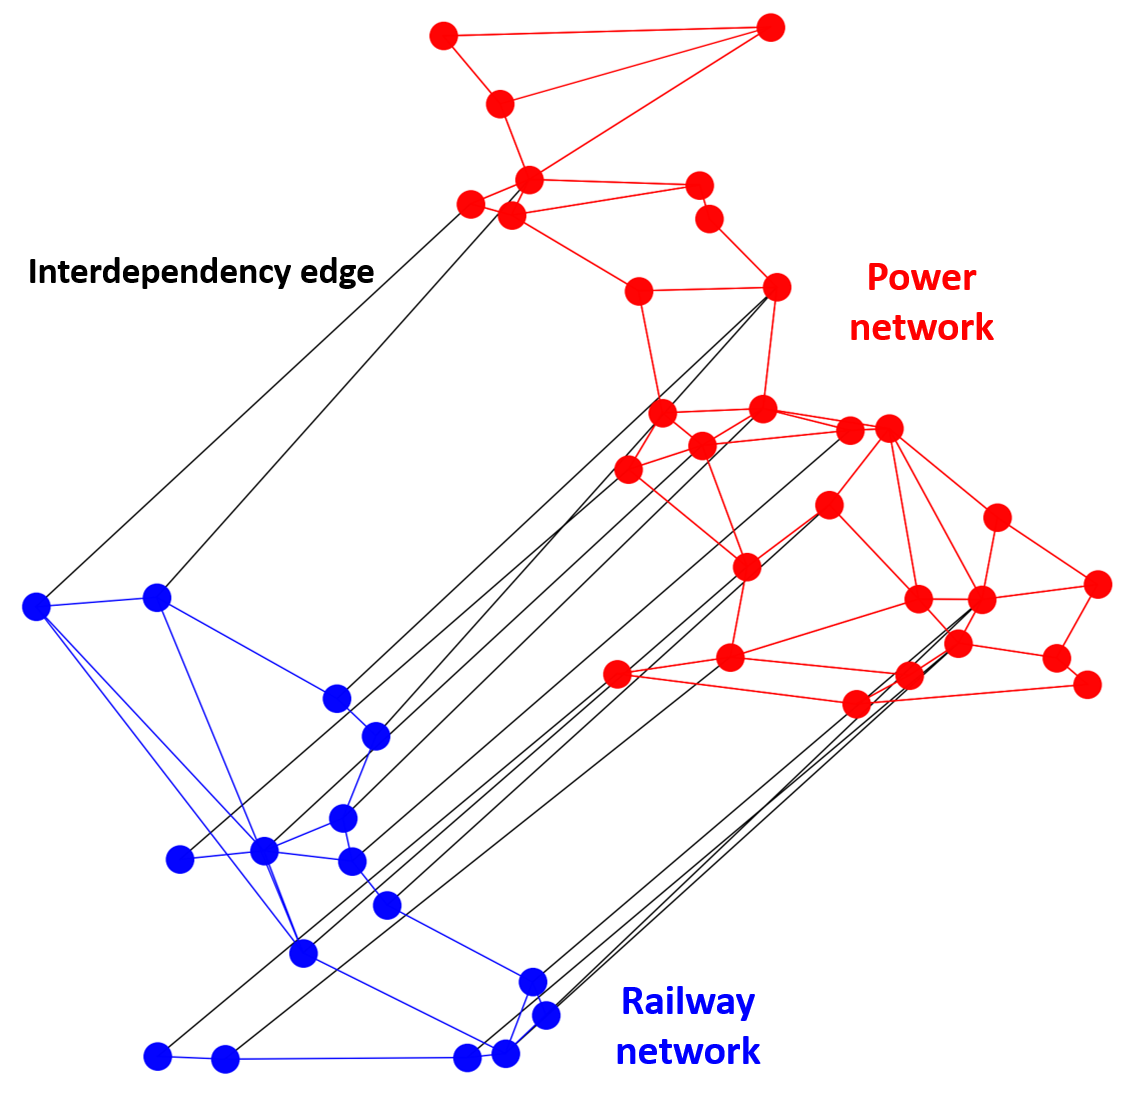
\includegraphics[width=6cm]{ images/NoN.png}
	\caption{Representation of interdependent railway and power networks.}
	\label{NoN}
\end{figure}	

	\subsection{Modeling initiating events}
	Initiating events represent single and multiple failures which might affect a system during normal operation or external strains. Vulnerability analysis investigates the system's response to different initiating events, often modeled as removals of an increasing fraction of components from the network \cite{johansson2011vulnerability}\cite{pant2016vulnerability}. The set of components to remove is defined as $\mathbf{N_f}=\{ n_{f,1}, n_{f,2},...,n_{f,N_{fail}} \}$. The number of components $N_{fail}$ which constitute the set $\mathbf{N_f}$ depends on the fraction $f$ according to Equation \eqref{random_fail}:
    \begin{equation}
        N_{fail} = \lfloor f \cdot (N + M)  \rfloor
        \label{random_fail}
    \end{equation}
    where $N$ and $M$ are respectively the number of nodes and edges in the network and $\lfloor \cdot  \rfloor$ is the floor function which returns the greatest integer less than or equal to the argument of the function. As it is clear from Equation \eqref{random_fail}, we consider the set of $\mathbf{N_f}$ to be composed by nodes and edges. This is to reflect initiating events which might impact both the type of components. For example, in a power network, an extreme storm can cause disturbances in power plants (nodes) due to floods and failures of lines (edges) due to strong gust winds. When an edge fails, it is simply removed from the network. When a node fails, also the edges connected to it are removed. The fraction $f$ can be interpreted as the magnitude of the initiating event. The elements selection of the set $\mathbf{N_f}$ depends on the type of initiating event. In this work, we consider two types of removal strategies for initiating events: random removals and spatially-localized removals.
    
    Random removals represent a wide range of initiating events (human errors, structural defects, random sabotages, etc.), and they are useful for understanding the robustness of a network under different magnitude of strains which might impact multiple locations of the network. Given the set of network components $\mathbf{C} = \mathbf{V} \displaystyle \cup \mathbf{E}=\{ c_1,c_2,...,c_{N+M} \} $ (either of railway or power network), we assume that each component, either node or edge, has the same probability $p_{ie}$ of being selected as part of the initiating and removed, computed according to Equation \eqref{p_ie_random}:
    \begin{equation}
    p_{ie} = \frac{1}{M+N}.
        \label{p_ie_random}
    \end{equation}
    The component selection is made according to Equation \eqref{selec_random} and the procedure shown in Figure \ref{algo_ie}:
    
    \begin{equation}
        p_{ie} \cdot (i-1) \le r < p_{ie} \cdot i
        \label{selec_random}
    \end{equation}
    where $0<r<1$ is a random number and $i$ is the index of the component $c_i$ which satisfies the above relationship. A component $c_i$ represents the node $v_i$ if $i\le N$, or the edge $e_{i-N}$ if $i>N$.
    
\begin{figure}[h]
	\centering
	\rotatebox{0}{
\includegraphics[width=5cm]{images/algo_ie.png}}
	\caption{Flowchart of the algorithm for the initiating event selection.}
	\label{algo_ie}
\end{figure}
    


   
    In spatially-localized removals, a fraction of components which belong to a specific geographical region or location is removed from the network. Spatially-localized removals are a good representation of damages caused by extreme weather events, like storms and floods, which are usually confined within a delimited geographical space. The selection procedure for the set of initiating failures is similar to the previous one, except for the set of components used for the initial event selection. We define $\mathbf{V^{reg}_{i}}=\{ v^{reg}_{i,1}, v^{reg}_{i,2},...,v^{reg}_{i,N^{reg}_{i}} \}$ as the set of $N^{reg}_{i}$ nodes belonging to the region $i$ subjected to the localized attack and $\mathbf{E^{reg}_{i}}=\{ e^{reg}_{i,1}, e^{reg}_{i,2},...,e^{reg}_{i,M^{reg}_{i}} \}$ as the set of $M^{reg}_{i}$ edges connected to the aforementioned nodes. The components selection is performed using Equations \eqref{random_fail}, \eqref{p_ie_random}, \eqref{selec_random} and the procedure in Figure \ref{algo_ie}, replacing the full set of components $\mathbf{C} = \mathbf{V} \displaystyle \cup \mathbf{E} $, the number of nodes $N$ and the number of edges $M$ respectively with $\mathbf{C^{reg}_{i}} = \mathbf{V^{reg}_{i}} \displaystyle \cup \mathbf{E^{reg}_{i}} $, $N^{reg}_{i}$ and $M^{reg}_{i}$.

	\subsection{Modeling cascading failures}
	Cascading failure is defined as a \say{kind of failure in a system comprising interconnected parts, in which the failure of a part can trigger the failure of successive parts} \cite{mahmoud2019networked}. We thus refer as cascading failures to the process of failure propagation within and between networks, triggered by an initiating event. Simulating cascading failures is an iterative simulation process. At each step, the network topology is updated, as failed components are removed. The general procedure for cascading failures simulation in single or interdependent networks includes the following steps:
        \begin{enumerate}
            \item Initialize network $\mathbf{G}=(\mathbf{V},\mathbf{E})$.
            \item Initialize initiating event $\mathbf{N_f}$.
            \item Remove failed elements.
            \item Update network topology.
            \item Check conditions for cascading failures.
            \item If there is any new failure, go back to step 3; otherwise, stop the simulation.
 \end{enumerate}
In the developed framework, three types of cascading failures are modeled: within the railway network, within the power network and between networks (from the power network to the railway network).
	\subsubsection{Cascading failures within railway networks}
	In the railway network, we refer as cascading failures to the process of stations and railways disconnection from the rest of the network.
	
	A station $i$ is considered to be functional if it si connected to at least another station with a railway. We define $\mathbf{N_{s,i}} = \{ v_{r,1}, v_{r,2},...,v_{r,N_{s,i}} \}$ as the set of $N_{s,i}$ stations directly connected through an edge to station $i$. If $\mathbf{N_{s,i}}$ is an empty set, station $i$ is considered disconnected and failed. This condition is formalized in Equation \ref{casc_rail_node}:
	\begin{equation}
	     S^r_{s,i} =
  \begin{cases}
    1, & \text{if $\mathbf{N_{s,i}} \ne \emptyset$}\\
    0, & \text{otherwise}
  \end{cases}
  \label{casc_rail_node}
	\end{equation}
where $S^r_{s,i}$ represents the binary state of station $i$ (1 if functional, 0 if failed).

	A railway $i$ is considered to be functional if it is connected to two stations. We define $\mathbf{N_{rw,i}} = \{ v_{r,j}, v_{r,k} \}$ as the set of stations $j$ and $k$ connected by railway $i$. If $\mathbf{N_{rw,i}}$ does not contain two elements, railway $i$ is considered to be disconnected and failed. This condition is formalized in Equation \ref{casc_rail_edge}:
		\begin{equation}
	     S^r_{rw,i} =
  \begin{cases}
    1, & \text{if $\mathbf{|N_{rw,i}}|=2$}\\
    0, & \text{otherwise}
  \end{cases}
  \label{casc_rail_edge}
	\end{equation}
where $S^r_{rw,i}$ represents the binary state of railway $i$ (1 if functional, 0 if failed) and $|\cdot|$ is the set cardinality, or the number of elements contained by the set.

The iterative simulation procedure for cascading failures in railway networks is shown in Figure \ref{algo_rail}.
\begin{figure}[h]
	\centering
	\rotatebox{0}{
\includegraphics[width=8cm]{images/algo_rail.png}}
	\caption{Flowchart of the cascading failures algorithm for power networks.}
	\label{algo_rail}
\end{figure}
After the initialization of the railway network $\mathbf{G_r}=(\mathbf{V_r},\mathbf{E_r})$ and the initiating event $\mathbf{N_f}$, the components in $\mathbf{N_f}$ are removed from the network (each node is removed along with the connected edges). The network topology is updated and the remaining stations and railways are checked for possible disconnections using Equations \eqref{casc_rail_node} and \eqref{casc_rail_edge}. If new failures occur, the simulation goes back to step 3 in Figure \ref{algo_rail}; otherwise, the simulation is stopped. The output of the cascading failures simulation is the new railway network topology $\mathbf{G_r'}=(\mathbf{V_r'},\mathbf{E_r'})$
	
	\subsubsection{Cascading failures within the power network}
	The cascading failures mechanism differs considerably in power networks, since power generation and demand and power flows are factors which strongly contribute to the cascading dynamics. Following the contingency of one or more edges (transmission lines) or the failure of one or more nodes (electrical buses), the power network might endure a failure propagation process, due to different causes (e.g. overloads of transmission lines, disconnections, frequency change). Different models are available to simulate this behaviour (see \cite{guo2017critical} for a comprehensive literature review). Dynamics models based on power flow computations represent one of the most realistic approaches currently available. In this work, we rely on a flow-based model inspired by the fast-dynamics of the ORNL-PSerc-Alaska (OPA) model \cite{dobson2001initial,carreras2002critical,carreras2013validating}. This approach is based on the DC power flow model (see appendix for details) and linear optimization for the economic dispatch, and the main driver of the cascading failures is the overload of lines. The purpose of the model is to simulate the behaviour of a power network after the initial failure of one or more components, taking into account power production and consumption, power flows and operator actions. A power network $\mathbf{G_p}=(\mathbf{V_p},\mathbf{E_p})$ contains a set of generators $\mathbf{N_G}$, which represents the power production units, and a set of loads $\mathbf{N_L}$, which represents the power consumption units (users/consumers). Generators have positive power, while loads have negative power, and they are described in the sets of generators and loads power, respectively $\mathbf{P_G} = \{ P_{G,1}, P_{G,2},...,P_{G,N_G}  \}$ and $\mathbf{P_L} = \{ P_{L,1}, P_{L,2},...,P_{L,N_L}  \}$. Following the failure of one or more components, the topology of the power network changes, possibly along with the power production capacity and the total power demand (when an electrical bus fails, it is removed along with its generators, loads and connected lines). Given these changes, grid operators can act in order to maximize the power delivered to loads (or, in other words, minimize the load shedding) while minimizing the power production cost and respecting the main grid constraints, like power production capacities, power demands and line flow capacities. This process is simulated with the iterative simulation described by the flowchart in Figure \ref{new_opa}.
\begin{figure}[h]
	\centering
	\rotatebox{0}{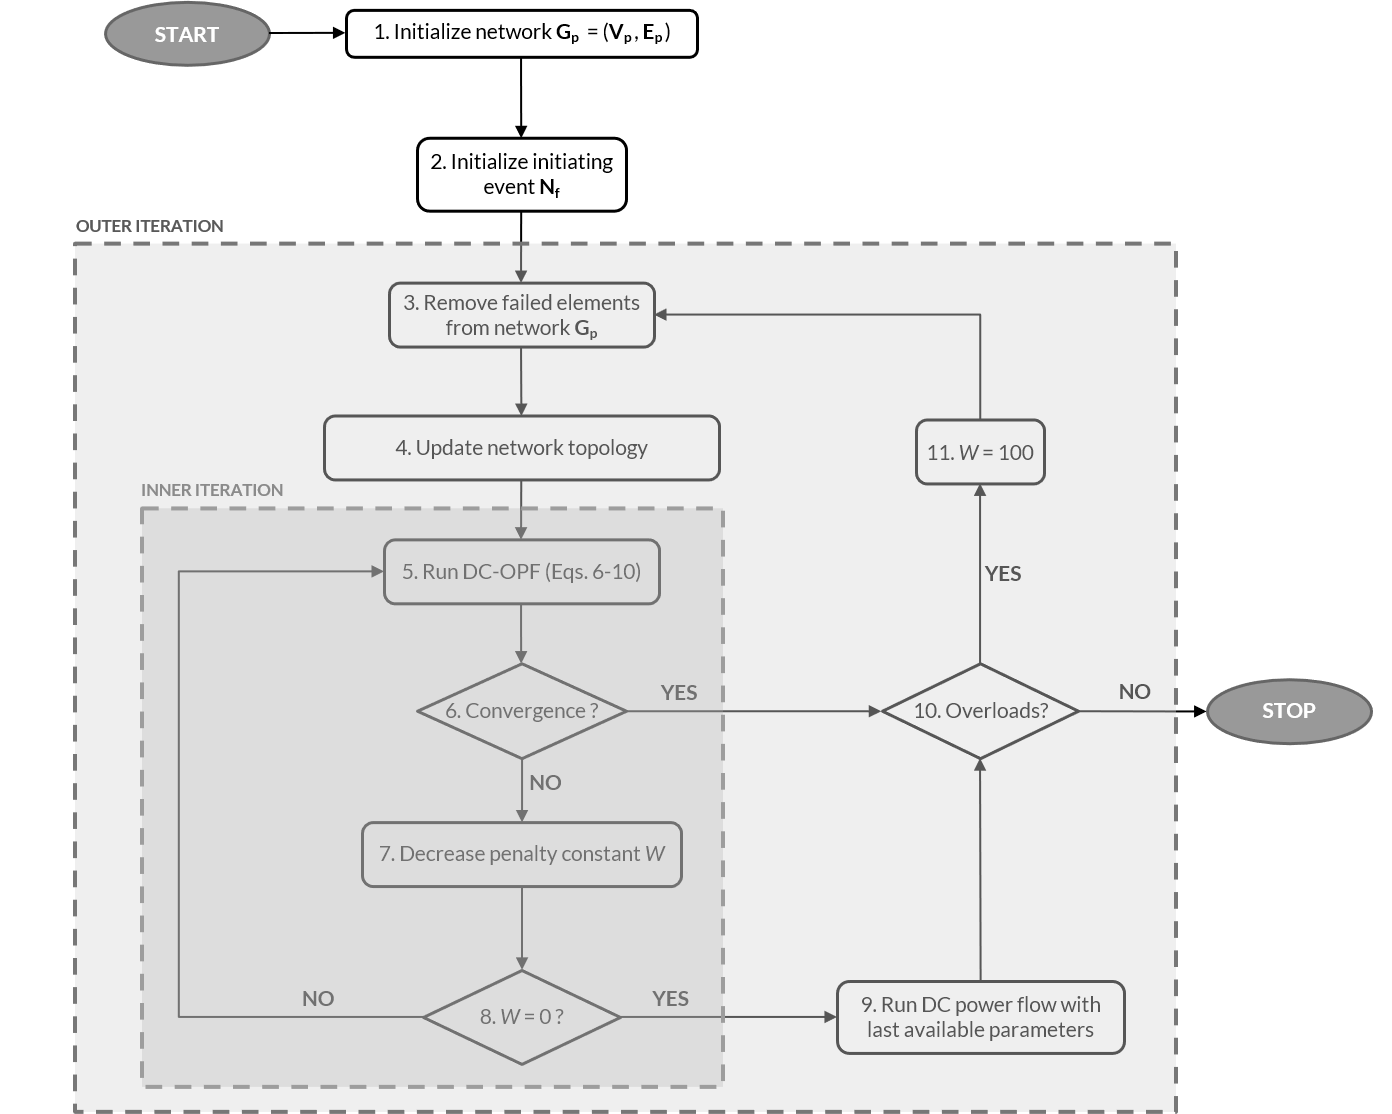
\includegraphics[width=12cm]{images/algo_opa.png}}
	\caption{Flowchart of the cascading failures algorithm for power networks.}
	\label{new_opa}
\end{figure}
	After the initialization of a power network $\mathbf{G_p}=(\mathbf{V_p},\mathbf{E_p})$ and the set of initial failures $\mathbf{N_f}$, the components in $\mathbf{N_f}$ are removed from the network, and the topology is updated. A change in topology will likely change the network performance, in terms of power produced and consumed at the nodes and distributed along the lines. Grid operators can then take an action to optimize the network functionality. This action is simulated with the linear optimization problem in Equations \eqref{cost_opa}-\eqref{line_flow_opa}:
	\begin{equation}
	\min_{\mathbf{P_G,P_L}} \;\;\; \sum_{i=1}^{N_G} P_{G,i} -W \sum_{j=1}^{N_L} |P_{L,j}|
	\label{cost_opa}
	\end{equation}
	
	\begin{equation}
	\sum_{i=1}^{N_G} P_{G,i} - \sum_{j=1}^{N_L} |P_{L,j}| = 0
	\label{power_balance_opa}
	\end{equation}
	\begin{equation}
	0 \le P_{G,i} \le P_{G,i}^{max}
	\label{generator_power_opa}
	\end{equation}
	\begin{equation}
	P_{L,j}^{max} \le P_{L,j} \le 0
	\label{load_power_opa}
	\end{equation}
	\begin{equation}
	-F_{l,k}^{max} \le F_{l,k} \le {l,k}l^{max}
	\label{line_flow_opa}
	\end{equation}
	where Equation \eqref{cost_opa} represents the cost function to minimize. The decision variables are the power at each generator and load, respectively represented by the sets $\mathbf{P_G}$ and $\mathbf{P_L}$. The first term of the equation represents the power production cost, which is assigned a unitary value per unit of power $P_{G,i}$ produced in each generator $i$. The second term represents the negative cost associated to the power $P_{L,i}$ supplied at each load $i$. The penalty constant $W$, here assumed to be equal to 100, ensure the minimization of load shedding when possible. Equations \eqref{power_balance_opa}-\eqref{line_flow_opa} represent the optimization constraints. The constraint in Equation \eqref{power_balance_opa} represents the power balance of generation and demand in the power network, which must be always equal to 0. Equations \eqref{generator_power_opa} and \eqref{load_power_opa} represents possible ranges of power of each generator and load. The constraint in Equation \eqref{line_flow_opa} represents the maximum power flow in each transmission line. The power flow in each line $F_l$ is computed using the DC power flow model (see appendix for details). This procedure is referred to as DC optimal power flow (DC-OPF), and it provides, as output, the decision variable sets $\mathbf{P_G}$ and $\mathbf{P_L}$ and the associated set of line power flow $\mathbf{F_l} = \{ F_{l,1}, F_{l,2},...,F_{l,M_p}  \}$. 
 In order to limit the computational time, the optimization is performed with the Python package Pandapower v. 2.4.0 \cite{pandapower.2018}, which utilizes an interior point solver for the DC-OPF. With this approach, the numerical convergence of the linear optimization is not always guaranteed. To overcome this problem, the inner iteration shown in Figure \ref{new_opa} is utilized. When a DC-OPF does not converge, the penalty constant $W$ is decreased (in this work, we decrease it by 2 units at each step), and a new DC-OPF is performed. This process is performed iteratively until a convergence is reached or the constant reaches the value 0, because a further decrease of the constant $W$ would lead to an optimization problem which aims to minimize power production. When $W=0$, a simple DC power flow computation with the last available parameters for $\mathbf{P_G}$ and $\mathbf{P_L}$ (for example, from a previous outer iteration) is performed. After a power flow computation, either optimal or not, the transmission lines are checked for possible overloads. In the traditional OPA model, a line is considered overloaded when its power flow is within 1\% of the maximum capacity of the line. An overloaded line is assumed to trip, and thus fail, with probability $p$. In this work, aiming for a conservative worst-case analysis, we assume $p=1$ \cite{cupac2013comparing}. The state of transmission line $k$ after a power flow computation is thus defined by Equation \eqref{state_line}:
 
 	\begin{equation}
	     S^p_{l,k} =
  \begin{cases}
    1, & \text{if $\frac{F_{l,k}}{F_{l,k}^{max}} < 0.99$}\\
    0, & \text{otherwise}
  \end{cases}
  \label{state_line}
	\end{equation}
where $S^p_{l,k}$ is the state of line $k$, $F_{l,k}$ the power flow at line $k$ and $F_{l,k}^{max}$ the maximum power flow capacity of line $k$. If some lines are overloaded, they are removed from the network, the penalty constant $W$ is set back to a value of 100 and a new outer iteration of the procedure is performed; otherwise, the simulation is stopped. The output of the cascading failures model is the new network topology $\mathbf{G_p'}=(\mathbf{V_p'},\mathbf{E_p'})$ and the new sets of generator and load power, defined as $\mathbf{P_G'} = \{ P_{G,1}', P_{G,2}',...,P_{G,N_G}'  \}$ and $\mathbf{P_L'} = \{ P_{L,1}', P_{L,2}',...,P_{L,N_L}'  \}$.

\subsubsection{Cascading failures between networks}

Since the power network supplies the necessary electricity to the railway network, disturbances in the former can propagate within the latter. Each station receives the electricity from the closest electrical bus containing a load in the power network, as defined by the set of interdependency edges $\mathbf{E_{r \leftarrow p}}$. Given the interdependency $e_{r \leftarrow p}^{i \leftarrow j,k}$, the station $i$ is supplied by the electrical bus $j$ containing the load $k$, which represents the power demand of $i$. Let $P_{L,k}$ and $P_{L,k}'$ represent the power supplied to load $k$ respectively before and after a disruptive event (for example an initiating event with consequent cascading failures). To model the tolerance of station $i$ against load shedding, let us introduce $R_{P_L,k}$: 
\begin{equation}
    R_{P_L,k} = \frac{P_{L,k}'}{P_{L,k}}.
    \label{ratio_pl}
\end{equation}
The physical meaning of $R_{P_L,i}$ is the load shedding at load $k$, measured as the fraction of nominal power demand at load $k$ satisfied after a disruptive event. Given the interdependency $e_{r \leftarrow p}^{i \leftarrow j,k}$, we model the binary functional state of station $i$ according to Equation \eqref{tpi}:
\begin{equation}
 S^r_{s,i} =
  \begin{cases}
    1, & \text{if $R_{P_L,k} \ge T_{r \leftarrow p}^{P_L}$ and $0<T_{r \leftarrow p}^{P_L}\leq 1$} \\
    0, & \text{if $R_{P_L,k}<T_{r \leftarrow p}^{P_L}$ and $0<T_{r \leftarrow p}^{P_L}\leq 1$} \\
    0, & \text{if $R_{P_L,k}=T_{r \leftarrow p}^{P_L}$ and $T_{r \leftarrow p}^{P_L}=0$}
  \end{cases}
  \label{tpi}
\end{equation}
where $S^r_{s,i}$ represents the state of the station $i$ (1 if functional, 0 if failed) supplied by load $k$ and $0 \le T_{r \leftarrow p}^{P_L} \le 1$ represents the minimum fraction of satisfied power demand for station $i$ to be functional. When $T_{r \leftarrow p}^{P_L}=1$, it represents a \say{zero-tolerance} situation, where a station and the connected railways are considered to be functional only as long as the entire power demand is satisfied. When $T_{r \leftarrow p}^{P_L}=0$, it represents the opposite situation, where a station and the connected railways are functional as long as some electricity is provided. The case $0 < T_{r \leftarrow p}^{P_L} < 1$ represents situations in-between, where a station is considered functional as long as at least a specific fraction of the power demand is satisfied.
\begin{figure}[h]
	\centering
	\rotatebox{0}{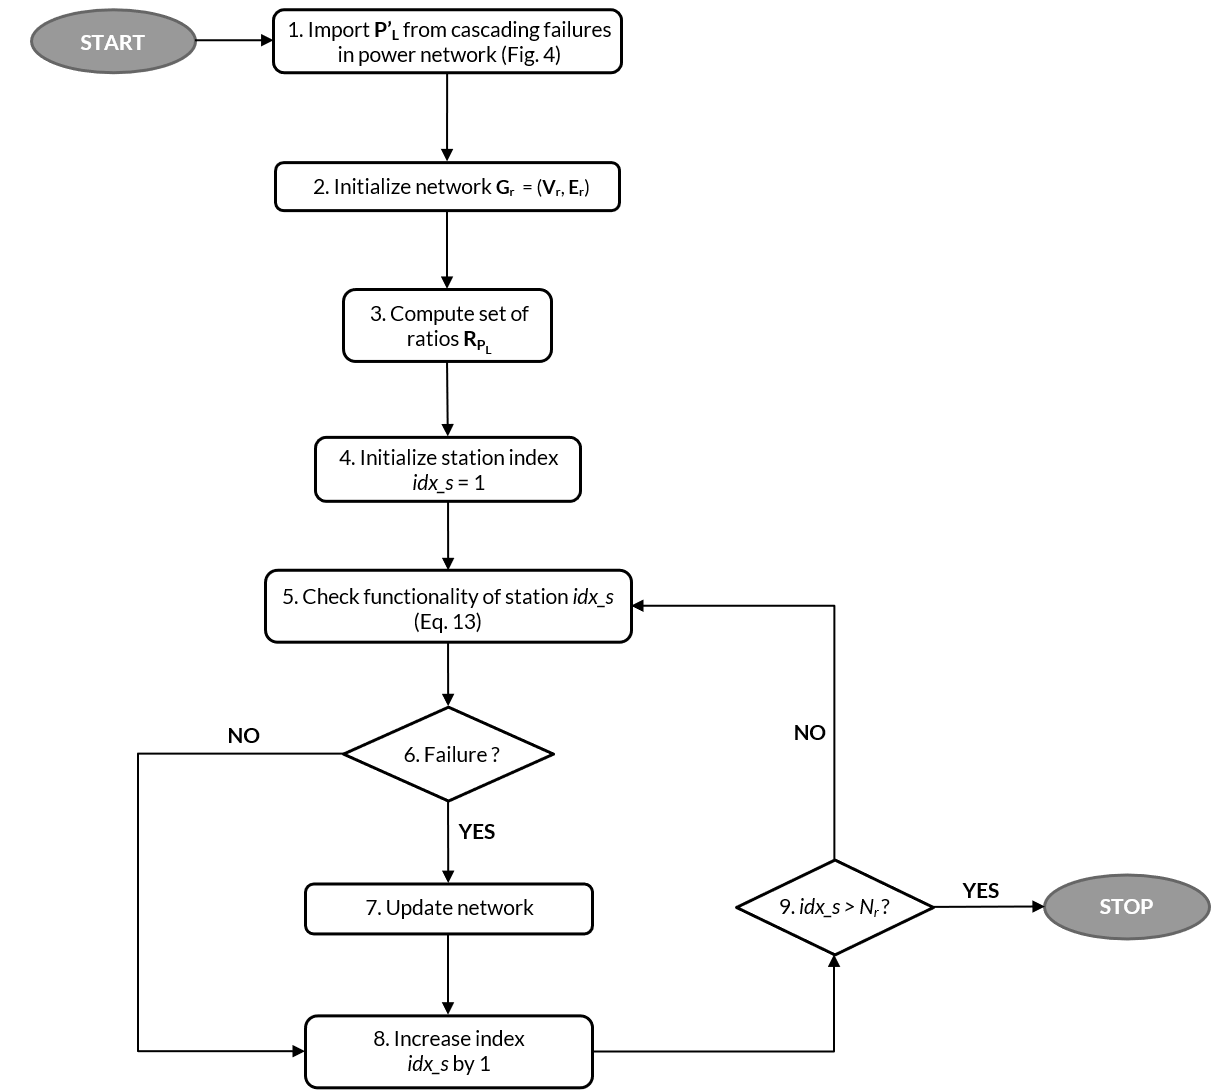
\includegraphics[width=12cm]{images/algo_between.png}}
	\caption{Flowchart of the cascading failures algorithm from power networks to railway networks.}
	\label{algo_bet}
\end{figure}
The flowchart of the algorithm for the cascading failures from power networks to railway networks is shown in Figure \ref{algo_bet}. The simulation starts importing the set $\mathbf{P_L'}$, which represents the power supplied at each load after a disruptive event, computed with the algorithm in Figure \ref{new_opa}. The railway network is then initialize and the set of ratio $\mathbf{R_{P_L}} = \{ R_{P_L,1}, R_{P_L,2},...,R_{P_L,N_L}   \}$ is computed using Equation \ref{ratio_pl} for each load. The functionality of each station is checked according to Equation \ref{tpi}, taking into account the interdependencies between stations and loads denoted in $\mathbf{E_{r \leftarrow p}}$. When a station fails, it is removed along with the connected railways and the network topology is updated. The algorithm stops when all the stations have been checked, and the output is the new railway network topology $\mathbf{G_r'}=(\mathbf{V_r'},\mathbf{E_r'})$.

	\subsection{Vulnerability}
	Vulnerability analysis aims at estimating the negative consequences which arise in a system given an imposed strain \cite{johansson2013reliability}. 
	Mathematically, the negative consequences on a system can be defined as the relative change of a specific performance indicator after a disruptive event, and the vulnerability $V$ can be generally expressed as in Equation \eqref{vulnerability_general}:
	\begin{equation}
	V = \frac{PI-PI'}{PI}
	\label{vulnerability_general}
	\end{equation}
	where \textit{PI} and \textit{PI}$'$ represent respectively the performance indicator before and after the disruptive event. The performance indicator is selected according to the type of system under analysis. For the railway network, the performance indicator used in this work is the accessibility $A_{r}$, expressed in Equation \eqref{access}:
	\begin{equation}
	A_r = \frac{1}{N_r}\sum_{i=1}^{N_r} \frac{n_{a}^i}{N_r-1}
	\label{access}
	\end{equation}
	where $N_r$ is the total number of stations and $n_{a}^i$ is number of stations accessible from the station $i$. It can be interpreted as the average fraction of stations accessible from (or connected to) each other \cite{ouyang2014comparisons}.\\
	For the power network, the performance indicator used in this work is the ratio between the actual power demand satisfied and the total power demand of loads after a disruptive event, here defined as Fraction of Demand Not Supplied (FDNS), as visible in Equation \eqref{edns}:
	\begin{equation}
	FDNS = \frac{\sum_{i=1}^{N_L} P_{L,i} -  \sum_{i=1}^{N_L} P_{L,i}'}{\sum_{i=1}^{N_L} P_{L,i}}.
	\label{edns}
	\end{equation}
	where $P_{L,i}$ and $P_{L,i}'$ represent respectively the power supplied to the load $i$ before and after a disruptive event.

	
	\section{Case-study and simulation approach}
	The developed model is applied to investigate the impact of interdependencies on the vulnerability of a electrified railway network. For this, a simplified version of a British high-speed railway system, based on a proposition made in \cite{greengauge2009fast}, is considered. The system comprises a railway network powered by an external power network. The railway network consists of 16 stations connected by 21 railways. The power network is based on the Great Britain reduced power network \cite{bukhsh2013network}. It consists of 29 electrical buses, containing 29 loads (one in each bus) and 66 generators, and connected by 99 lines, most of them in redundant double circuit configuration. As it was aforementioned, it is assumed that the electricity is supplied to each station from the closest electrical bus containing a load, which represents the power demand of the corresponding station, as denoted by the set of interdependency edge $\mathbf{E_{r \leftarrow p}}$. The interdependencies are shown in Table \ref{interdependencies}.
	\begin{table}[h]
		\centering
		\caption{One-to-one unidirectional interdependencies between railway and power network, correpsonding to the set of interdependency edge $\mathbf{E_{r \leftarrow p}}=\{ e_{r \leftarrow p}^{i \leftarrow j,k}, e_{r \leftarrow p}^{h \leftarrow v,u},...,e_{r \leftarrow p}^{N_r \leftarrow N_p, N_L} \}$. Since there is one load for each bus, the bus index $j$ and the load index $k$ are the same.}
		\begin{tabular}[t]{lclc}
			\hline
			\textbf{Station ($i$)}& \textbf{Bus/load} & \textbf{Station ($i$)}& \textbf{Bus/load}\\
			\hline
			Glasgow (1) & 4 & Stansted (9) & 20 \\
			Edinburgh (2) & 3 & London (10) & 24\\
			Newcastle (3) & 9 &  Heathrow (11)  &  24\\
			Tees Valley (4) & 9 & Bristol (12) & 22\\
			Leeds (5) & 14 & Cardiff (13) & 28\\
			Sheffield (6) & 13 & Birmingham (14) & 17\\
			Nottingham (7) & 16 & Manchester (15) & 12\\
			Cambridge (8) & 20 & Liverpool (16) & 11\\
			\hline
		\end{tabular}
		\label{interdependencies}
	\end{table}%
	When two or more stations share the same load, the latter is assumed to represent the power demand of all the station connected. For example, the load at the bus 9 represents the power demand of the stations of Newcastle and Tees Valley. We assume the maximum power generation capacity to be slightly higher than the maximum power demand, respectively 57.29 GW and 56.32 GW. The generator power capacities range from 0.083 GW to 5.45 GW. The load power demands range from 0.117 GW to 9.734 GW. For other electrical parameters of the power network, please refer to the data available in \cite{bukhsh2013network}. The graphical representation of the two networks is shown in Figure \ref{regions}.
The developed modeling framework is used to analyze the vulnerability of the aforementioned railway and power network in three different scenarios:
\begin{enumerate}
\item Vulnerability of railway network due to random removals in the power network. This scenario allows to analyze the impact on the railway network of multiple random failures in the power network.
\item Vulnerability of railway network due to spatially-localized removals in the power network. This scenario allows to analyze the impact of multiple spatially-localized failures in the power network on other locations of the railway network.
\item Vulnerability of railway and power network due to random removals in both the two networks. This scenario allows to evaluate the impact on the railway and power network in the case of multiple random failures in both the networks.
\end{enumerate}
For each scenario, the cascading failures between networks is evaluated for three different values of $T_{r \leftarrow p}^{P_L}$ ( 0.0, 0.5 and 1.0). The different modeling features are combined in an iterative simulation algorithm which allows to perform a detailed vulnerability analysis. Each single iteration of the algorithm follows these main steps:
\begin{enumerate}
    \item Initialize networks and elements to remove.
    \item Remove failed elements.
    \item Simulate cascading failures.
    \item Compute vulnerabilities.
\end{enumerate}
	The simulation requires multiple iterations because different combinations of components in $\mathbf{N_f}$ leads to a different vulnerability values. For each of the three scenarios, we compute the vulnerabilities for increasing fractions of removals, from 0\% to 100\%, with steps of 10\%. At each level of removal fraction, the average value of the vulnerability is computed through 500 Monte Carlo simulations. Average values $\Bar{V}$ and 95\% confidence intervals $CI_{95}$ for each fraction of removals are computed respectively with Equation \eqref{average_mc} and \eqref{ci95}:
\begin{equation}
    \Bar{V} = \frac{\sum_{i=1}^{N_{exp}} V_i}{N_{exp}}   
\label{average_mc}
\end{equation}
\begin{equation}
    CI_{95} = \Bar{V} \pm Z*\frac{\sigma}{\sqrt{N_{exp}}} 
    \label{ci95}
\end{equation}
	where $N_{exp}$ is the number of experiments per fraction of removals, $Z$ is the 95\% confidence interval constant, equal to 1.96, and $\sigma$ is the standard deviation estimation.
	The flowchart of the algorithm for scenarios 1 and 2 is visible in Figure \ref{algo_scenario_1}. Firstly, fraction of removals, networks and initiating event are initialized. Secondly simulations of cascading failures in power network, between networks and in railway network are performed in this order (steps 6-8 in Figure \ref{algo_scenario_3}). Thirdly, vulnerabilities and confidence intervals are computed. This procedure is performed iteratively until reaching 500 simulations per fraction of removals. In this case, it is important to precise the nature of the relationship between stations and the corresponding loads. As it was previously described, we relate the state of station $i$ to the load shedding at load $k$ in bus $j$, according to the interdependency $e^{i \leftarrow j,k}_{r\leftarrow p}$ and Equation \ref{tpi}. Load $k$ does not represent exclusively the power consumed by station $i$, but it rather represents the power demand of multiple users in the area (including the connected stations). In scenario 1 and 2, rather than explicitly assigning a power demand to station $i$, we assume, without loss of generality, that the fraction of power demand satisfied at station $i$ is directly proportional to the fraction of total power demand satisfied at load $k$, whatever is the specific power demand of station $i$. For example, if the total load shedding at load $k$ is 50\%, we assume that station $i$ is supplied with 50\% of its power demand. This assumption is valid for scenarios 1 and 2, and they are both be analyzed using the algorithm in Figure \ref{algo_scenario_1}, but with two main differences:
    \begin{itemize}
        \item In scenario 1, the initiating event is selected from the total set of power network components $\mathbf{C_p} = \mathbf{V_p} \displaystyle \cup \mathbf{E_p}$, while in scenario 2 the set of power network components in region $i$ $\mathbf{C^{reg}_{p,i}} = \mathbf{V^{reg}_{p,i}} \displaystyle \cup \mathbf{E^{reg}_{p,i}}$ is used.
        \item The vulnerability of the railway network in scenario 1 is measured as loss of accessibility, while in scenario 2 it is measured simply as number of failed stations per region and in total. 
    \end{itemize}
    In scenario 2, the geographical space containing the elements of the networks is divided into six regions, as shown in Figure \ref{regions}. These six regions are defined in a qualitative graphical way. In this work, we do not account for the impact and the sensitivity analysis of different region sizes. The algorithm in Figure \ref{algo_scenario_1} must be performed for each one of the six regions.
\begin{figure}[h]
	\centering
	\rotatebox{0}{
\includegraphics[width=12cm]{images/algo_scenario_1.png}}
	\caption{Algorithm for the vulnerability analysis with random and spatially-localized removals in power network.}
	\label{algo_scenario_1}
\end{figure}
\begin{figure}[h]
	\centering
	\rotatebox{0}{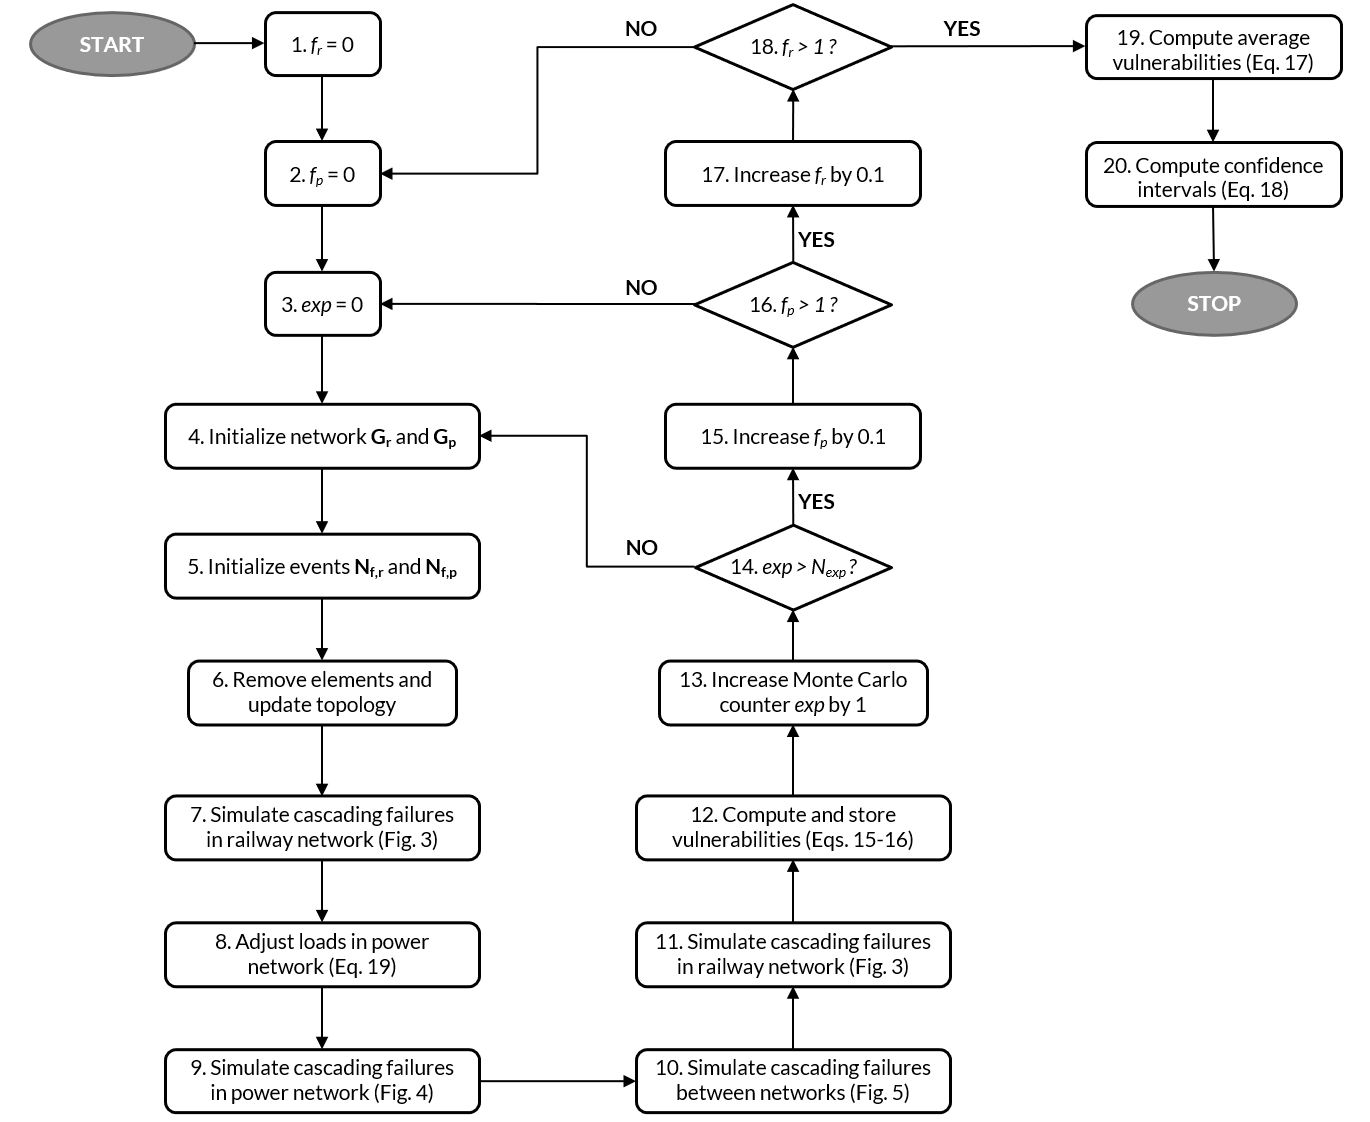
\includegraphics[width=12cm]{images/algo_simulation.png}}
	\caption{Algorithm for the vulnerability analysis with simultaneous removals in railway and power network. $f_r$ and $f_p$ are the fraction of elements to remove respectively in the railway network and in the power network; $\mathbf{N_{f,r}}$ and $\mathbf{N_{f,p}}$ are the sets of initiating event respectively in the railway network and in the power network; $N_{exp}$ is the maximum number of iterations for combination of fractions of removals (500 in this study).}
	\label{algo_scenario_3}
\end{figure}

    The flowchart of the algorithm used for the analysis of scenario 3 is shown in Figure \ref{algo_scenario_1}. Firstly, fractions for removals, networks and initiating events are initialized. Secondly, simulations of cascading failures in railway network, power network, between networks and railway network (steps 7-11 in Figure \ref{algo_scenario_3}) are performed. Thirdly, vulnerabilities and confidence intervals are computed. The vulnerabilities of railway and power network are computed respectively in terms of loss of accessibility and FDNS. Again, this procedure is repeated iteratively until 500 simulations per fraction of removals in power and railway network are performed. Contrary to the previous scenarios, given an interdependency $e^{i \leftarrow j,k}_{r\leftarrow p}$, we assume that load $k$ represents exclusively the power demand of station $i$. After the first cascading failures simulation in the railway network (step 6), and before running the cascading failures simulation in the power network (step 8), the power demand of each load is adjusted according to Equation \eqref{load_demand}:
\begin{equation}
P^{adj}_{L,i} =
  \begin{cases}
    P_{L,i} \frac{n'_s}{n_s}, & \text{if $n_s>0$} \\
    P_{L,i}, & \text{otherwise}
  \end{cases}
  \label{load_demand}
\end{equation}
	where $P^{adj}_{L,i}$ is the adjusted power demand of load $i$, $P_{L,i}$ is the nominal power demand of load $i$, and $n_{s,i}$ and $n'_{s,i}$ represent respectively the stations connected to load $i$ before and after the initiating removals and the cascading failures in the railway network. This assumption, despite being unrealistic and in contrast with the previous cases, allows to emphasize and generalize the effect of failures in the railway network, which can be generalized as a "consumer network", on the power network, generalized as a "producer/supplier network". This effect is magnified in terms of magnitude, but not modified in terms of behaviour. Further details are available in the next sections.
	
\begin{figure}[ht]
	\centering
	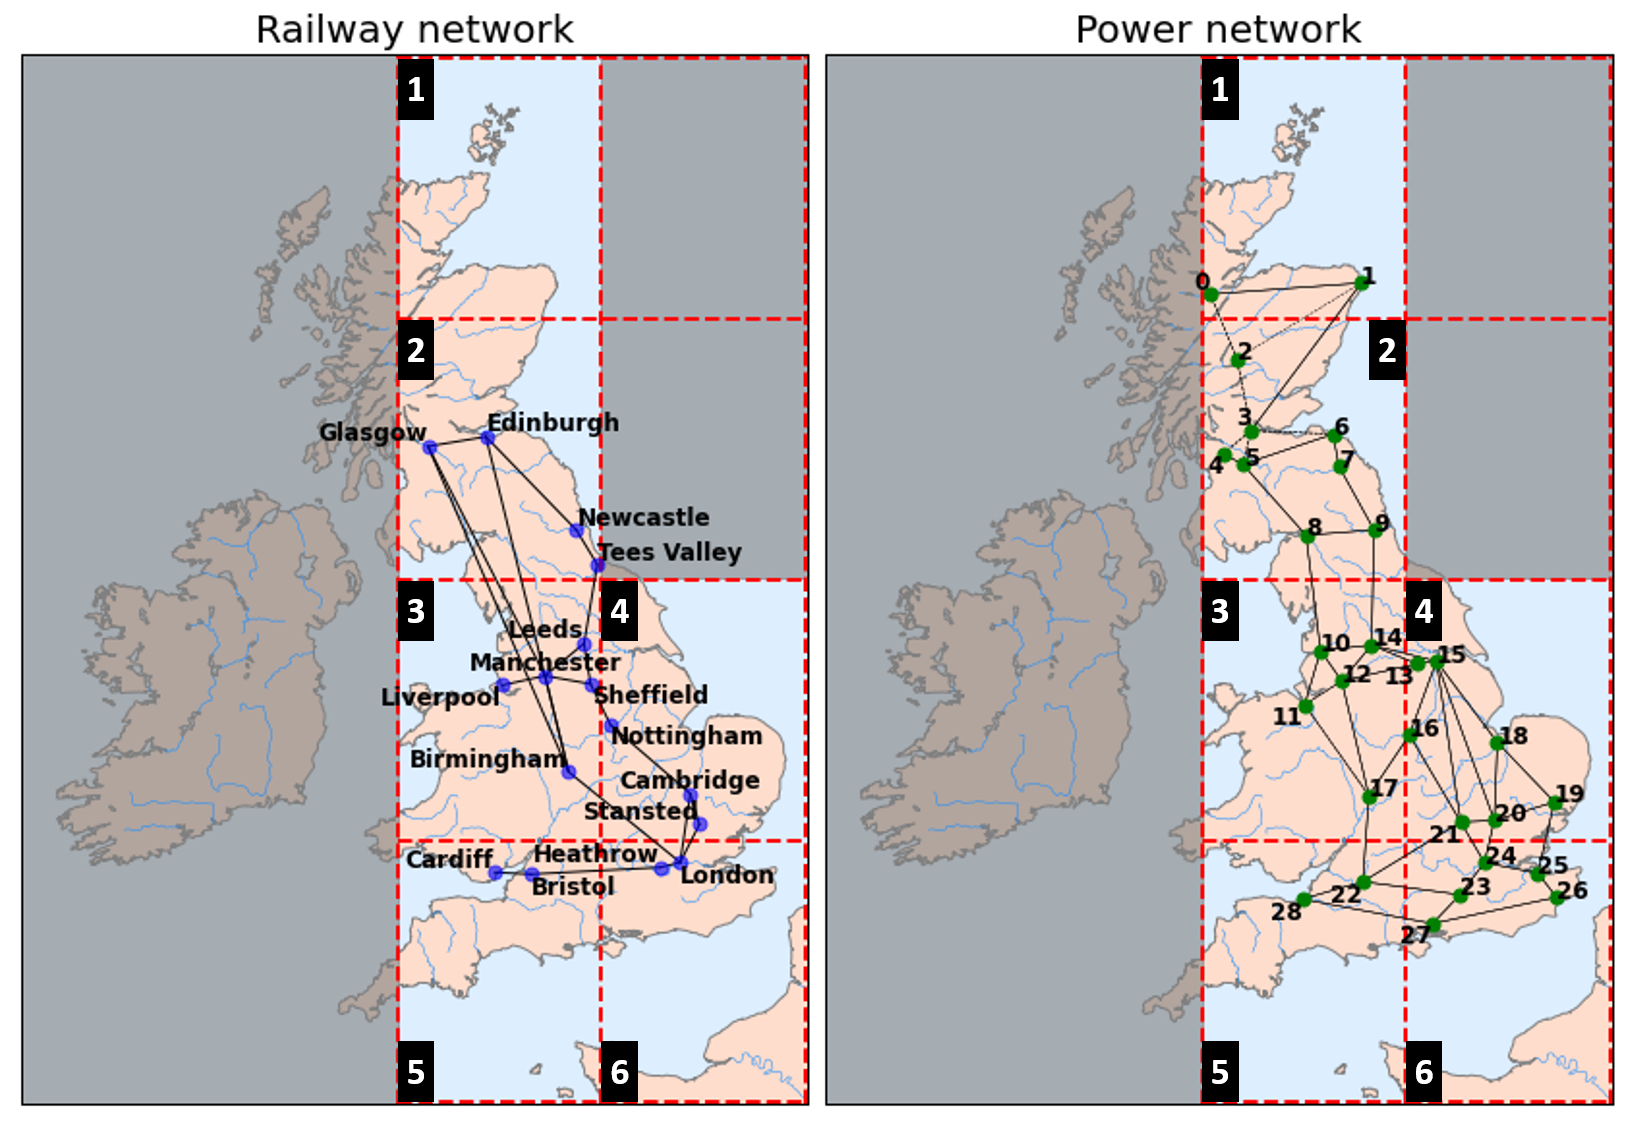
\includegraphics[width=8cm]{ images/regions_both.png}
	\caption{Representation of the six qualitative geographical regions utilized in this work and the corresponding elements in the railway and power network.}
	\label{regions}
\end{figure}

	
	\section{Results}
	\subsection{Scenario 1: random removals in power network}
	\subsubsection{The impact of the power network on the railway network}
	
	A specific fraction of elements (from 0\% to 100\%, with steps of 10\%), either nodes or edges, is randomly removed from the power network. Through the model described in the previous section, the ratio $R_{P_L,k}$ for each load is computed. This value is used to evaluate the electricity supply in the railway network. The impact on the railway network is assessed by the average loss of accessibility for three $T_{r \leftarrow p}^{P_L}$ values (0.0, 0.5 and 1.0). The results are presented in Figure \ref{vuln_power_to_rail}.
	
	As it can be clearly seen, the impact in the railway network follows different patterns as the threshold $T_{r \leftarrow p}^{P_L}$ changes. Intuitively, the lower is the threshold, the less vulnerable is the network. A direct measure of the disruption magnitude is the area below the vulnerability curves in Figure \ref{vuln_power_to_rail}. For comparison, the values of the areas below curves for $T_{r \leftarrow p}^{P_L}=0.5$ and $T_{r \leftarrow p}^{P_L}=0.0$ are computed and normalized with the area below the curve for $T_{r \leftarrow p}^{P_L}=1.0$. The results are respectively 0.90 and 0.87.
	
	With $T_{r \leftarrow p}^{P_L}=1.0$, a percentage of removals of 10\% of the elements in the power network is sufficient to lose almost a fraction of accessibility of 0.6 in the railway network. For the same percentage of removals, the loss of accessibility is just below 0.3 for both $T_{r \leftarrow p}^{P_L}=0.5$ and $T_{r \leftarrow p}^{P_L}=0.0$. In order to reach an average loss of accessibility of 0.99 in the railway network, the necessary percentages of removals are 70\%, 80\% and 90\%, respectively for $T_{r \leftarrow p}^{P_L}=1.0$, $T_{r \leftarrow p}^{P_L}=0.5$ and $T_{r \leftarrow p}^{P_L}=0.0$. 
		\begin{figure}[ht]
	\centering
	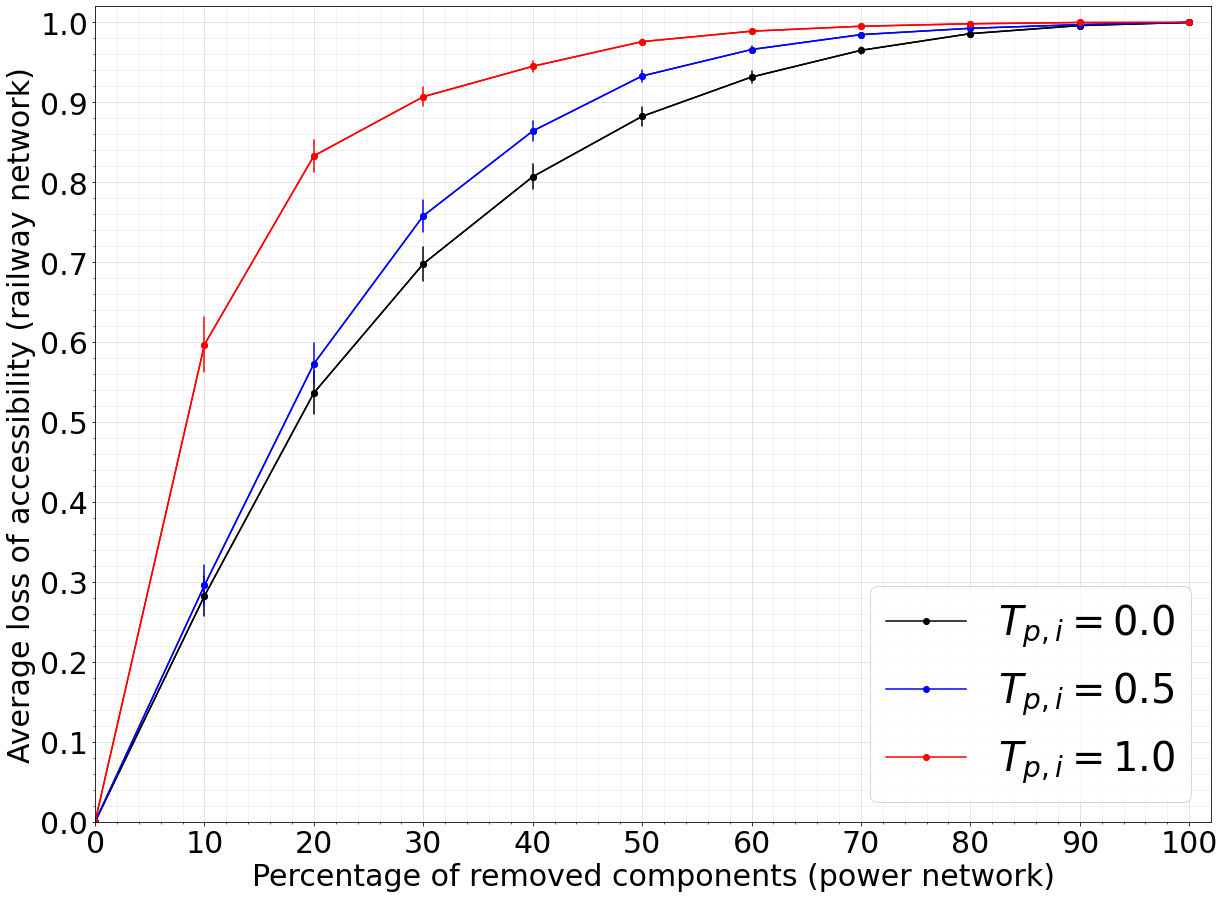
\includegraphics[width=8cm]{images/vuln_conn_power_to_rail.png}
	\caption{Average loss of accessibility in the railway network for different fraction of random removals in the power network. Results of 500 experiments per fraction of removals. 95\% confidence intervals are shown.}
	\label{vuln_power_to_rail}
\end{figure}

\subsubsection{The contribution of different failure modes}
We identify three main failure modes for a railway station:
\begin{enumerate}
	\item Load shedding due to direct removal: when the bus containing the corresponding load is failed due to direct removal, as part of the simulation of the initiating event. In other words, given the station $i$ failed due to cascading failures between networks (algorithm in Figure \ref{algo_bet}) and the interdependency $e^{i \leftarrow j,k}_{r\leftarrow p}$, the electrical bus $k$ is in the initiating event set $\mathbf{N_f}$.
	\item Load shedding due to cascading failures: when the load shedding in the corresponding load, computed with the cascading failures model, is due to any reasons other than the direct removal of the bus containing the load itself. In other words, given the station $i$ failed due to cascading failures between networks (algorithm in Figure \ref{algo_bet}) and the interdependency $e^{i \leftarrow j,k}_{r\leftarrow p}$, the electrical bus $k$ is not in the initiating event set $\mathbf{N_f}$.
	\item Station disconnection: when a station is disconnected from the rest of the railway network due to the failures of other stations. In other words, the station $i$ is failed due to cascading failures in the railway network (algorithm in Figure \ref{algo_rail}).
\end{enumerate}
		\begin{figure}[h]
	\centering
	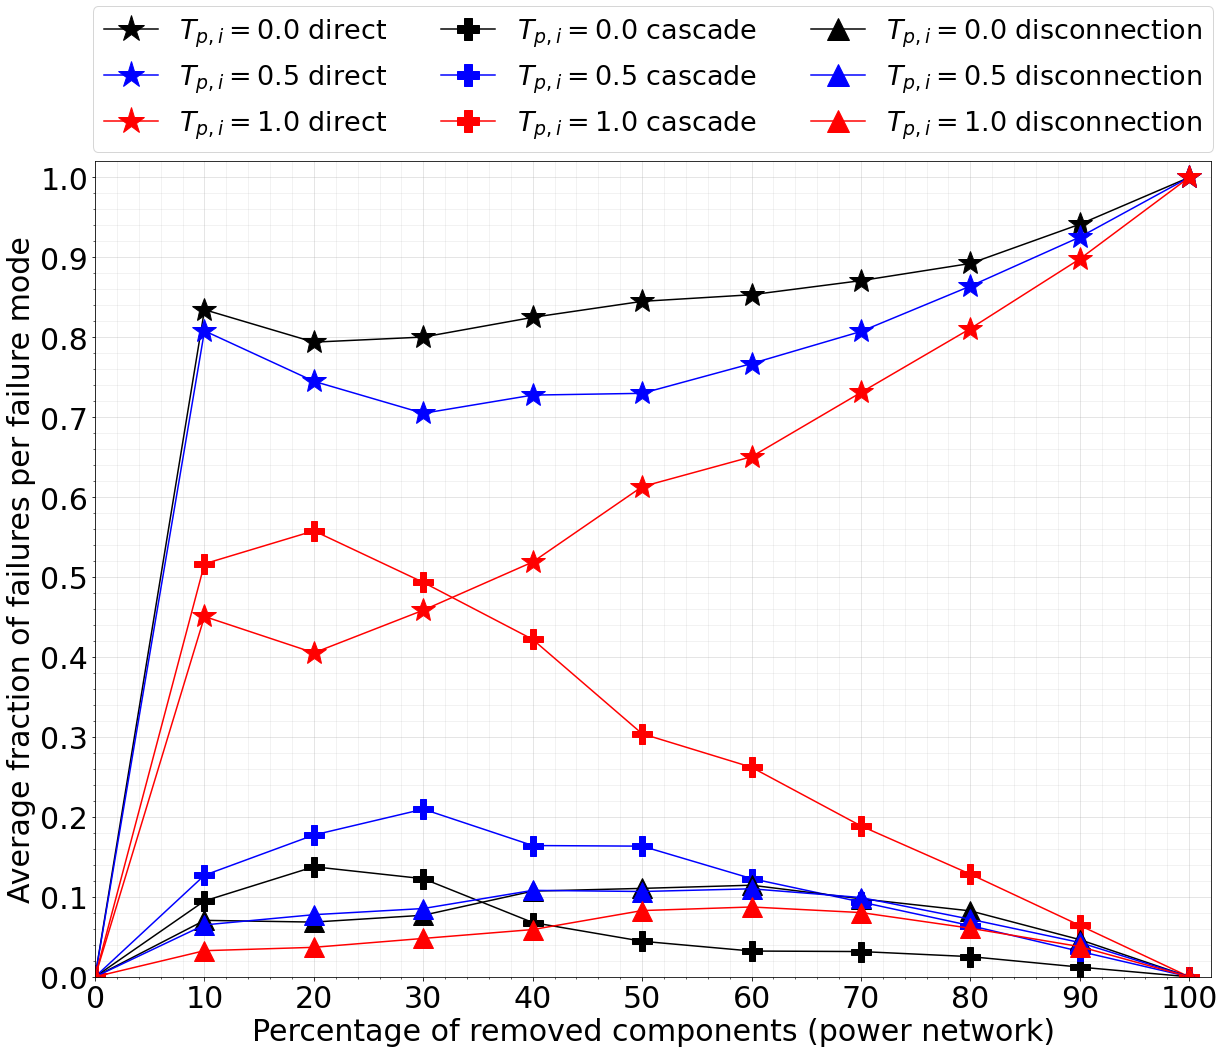
\includegraphics[width=8cm]{images/perc_fail_power_to_rail.png}
	\caption{Average fraction of failures in the railway network due to direct removal in the power network, disconnection in the railway network and cascading failures in the power network. Results of 500 experiments per fraction of removals. Confidence intervals are not shown for a clear visualization. The same color indicates the same threshold $T_{r \leftarrow p}^{P_L}$, while the same symbol indicates the failure mode.}
	\label{perc_fail_power_to_rail}
\end{figure}
In Figure \ref{perc_fail_power_to_rail} it is visible how the three failure modes contribute on average to the total failures in the railway network, expressed as the ratio between the station failed due to a specific failure mode over the total number of station failed.

The fractions of failures due to direct removals (failure mode 1, star symbol in Figure \ref{perc_fail_power_to_rail}) start with 10\% of removals at 0.45, 0.81 and 0.83 respectively for $T_{r \leftarrow p}^{P_L}=1.0$, $T_{r \leftarrow p}^{P_L}=0.5$ and $T_{r \leftarrow p}^{P_L}=0.0$. They then decrease, reaching their minimum with a percentage of removals between 20\% and 30\% (0.41 at 20\%, 0.70 at 30\%, 0.79 at 20\% respectively for $T_{r \leftarrow p}^{P_L}=1.0$, $T_{r \leftarrow p}^{P_L}=0.5$ and $T_{r \leftarrow p}^{P_L}=0.0$). They then increase monotonically, converging to 1.0 with 100\% of removals.

The fractions due to cascading failures (failure mode 2, cross symbol in Figure \ref{perc_fail_power_to_rail}) have an opposite trend. They start at 0.52, 0.13 and 0.09 respectively for $T_{r \leftarrow p}^{P_L}=1.0$, $T_{r \leftarrow p}^{P_L}=0.5$ and $T_{r \leftarrow p}^{P_L}=0.0$. They then increase, reaching the maximum with percentages of removals between 20\% and 30\% (0.56 at 20\%, 0.21 at 30\%, 0.14 at 20\% respectively for $T_{r \leftarrow p}^{P_L}=1.0$, $T_{r \leftarrow p}^{P_L}=0.5$ and $T_{r \leftarrow p}^{P_L}=0.0$). They then decrease monotonically to 0.0 with 100\% of removals. With $T_{r \leftarrow p}^{P_L}=0.5$ and $T_{r \leftarrow p}^{P_L}=0.0$, the fraction due to direct removals is always higher than the fraction due to cascading failures. With $T_{r \leftarrow p}^{P_L}=1.0$, the fraction due to cascading failures is higher than the one due to direct removals with a percentage of removals below 30\%. At a percentage of 30\%, the two fractions have similar values (between 0.45 and 0.5).

The fraction due to disconnection (failure mode 3, triangle symbol in Figure \ref{perc_fail_power_to_rail}) presents a non-monotonic trend. It increases until certain percentage of removals and then it decreases to 0. The maximum values are reached with 60\% of removals, and they are 0.09, 0.11 and 0.11 respectively for $T_{r \leftarrow p}^{P_L}=1.0$ , $T_{r \leftarrow p}^{P_L}=0.5$ and $T_{r \leftarrow p}^{P_L}=0.0$.

	
\subsection{Scenario 2: spatially-localized removals in power network}
The effect of spatially-localized random removals in the power network are evaluated for each region and threshold $T_{r \leftarrow p}^{P_L}$ and for fractions of removals from 0\% to 100\%, with steps of 10\%. Results for $T_{r \leftarrow p}^{P_L}=1.0$ , $T_{r \leftarrow p}^{P_L}=0.5$ and $T_{r \leftarrow p}^{P_L}=0.0$ are shown respectively in Figures \ref{regions_tp100}, \ref{regions_tp50} and \ref{regions_tp0}. Each plot shows the fraction of elements removed in a specific region (specified in the title of each plot) and the average number of stations failed in each region and in total. As it is clearly visible, the magnitude of the disruption strongly depends on the removals region and the assumption on $T_{r \leftarrow p}^{P_L}$. The greater is the threshold $T_{r \leftarrow p}^{P_L}$, and the greater is the disruption.

With $T_{r \leftarrow p}^{P_L}=1.0$, high levels of failure propagation between regions can be observed. The most critical regions are, in descending order and in terms of maximum number of failed stations in the whole network, region 2 (16 stations), region 4 (14 stations), region 3 (12 stations), region 1 (5 stations), region 5 (4 stations) and region 6 (4 stations). Moreover, regions 1, 2 and 3 shows a disruptive trend which increases monotonically, and the maximum level of disruption is reached when 100\% of elements are removed from the corresponding region. For regions 4,5 and 6, the maximum level of disruption is reached with lower fraction of removals, respectively 60\%, 60\% and 30\%.

With $T_{r \leftarrow p}^{P_L}=0.5$ and $T_{r \leftarrow p}^{P_L}=0.0$, the magnitude of disruption is generally lower due to the smaller contribution of cascading failures, as it can be seen in Figures \ref{regions_tp50} and \ref{regions_tp0}.




	
\subsection{Scenario 3: simultaneous random removals in both the networks}
Random removals in both the networks of fraction of elements from 0\% to 100\%, with steps of 10\%, are evaluated in terms of vulnerability analysis. The results for the railway and power network, in terms of loss of accessibility and FDNS, are visible respectively in Figure \ref{vuln_rail_ccf_100} and \ref{vuln_power_ccf_100}. Only the results for $T_{r \leftarrow p}^{P_L}=1.0$ are shown, since the other two cases present similar trends.

As expected, since the railway network is directly dependent on the power network, for a fixed fraction of removals $f_r$ in the railway network, removals in the power network lead to an increased level of disruption. This behaviour is clearly visible in Figure \ref{vuln_rail_ccf_100}. For example, the first row of the heatmap in Figure \ref{vuln_rail_ccf_100} corresponds to scenario 1 (red curve in Figure \ref{vuln_power_to_rail}). As it can be clearly seen, the average loss of accessibility is directly proportional to the values of $f_r$ and $f_p$.

On the contrary, random removals of elements in the railway network have a positive effect on the power network, as shown in Figure \ref{vuln_power_ccf_100}. For a fixed fraction of removals in the power network, the average FDNS decreases as the fraction of removals in the railway network increases. For example, for $f_p=20\%$ and $f_r=0\%$, the average FDNS is 0.41, while for $f_p=20\%$ and $f_r=100\%$ the average FDNS is 0.20. This trend is particularly accentuated for $20\% \le f_p \le 60\%$. In fact, with $f_p=10\%$, the average FDNS does not decrease monotonically with the increase of $f_r$. However, this is due to statistical errors (confidence intervals are not shown for a clear visualization) and the overall trend is decreasing. The same considerations are valid for $f_p \ge 70\%$.







	\begin{figure}[h]
	\centering
	\rotatebox{0}{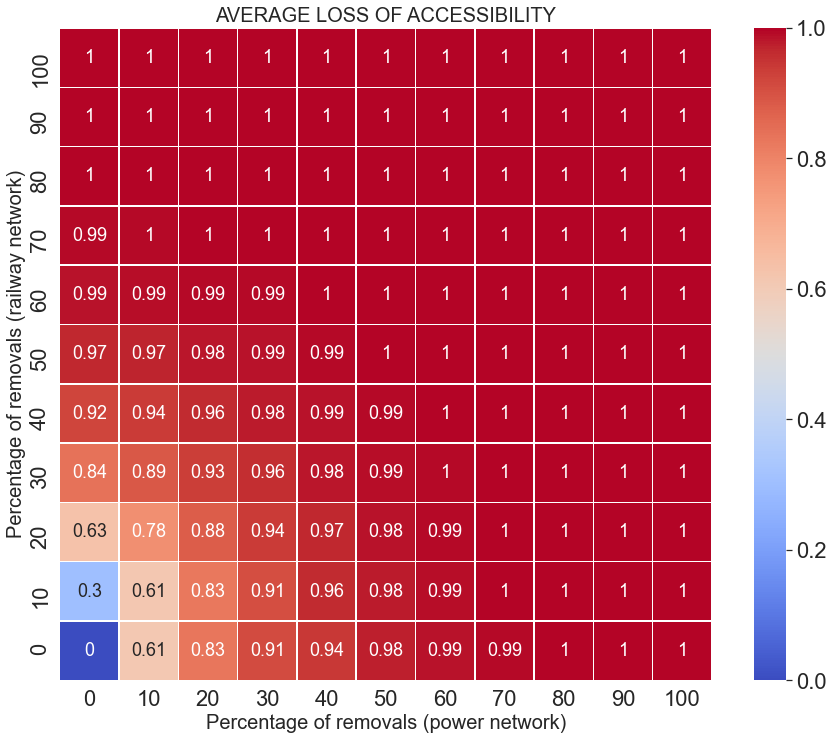
\includegraphics[width=8cm]{images/vuln_rail_ccf_100.png}}
	\caption{Vulnerability of the railway network with simultaneous random removals in both the networks and $T_{r \leftarrow p}^{P_L}=1.0$.Results of 500 experiments for fraction of removals. Confidence intervals are not shown.}
	\label{vuln_rail_ccf_100}
\end{figure}

\begin{figure}[h]
	\centering
	\rotatebox{0}{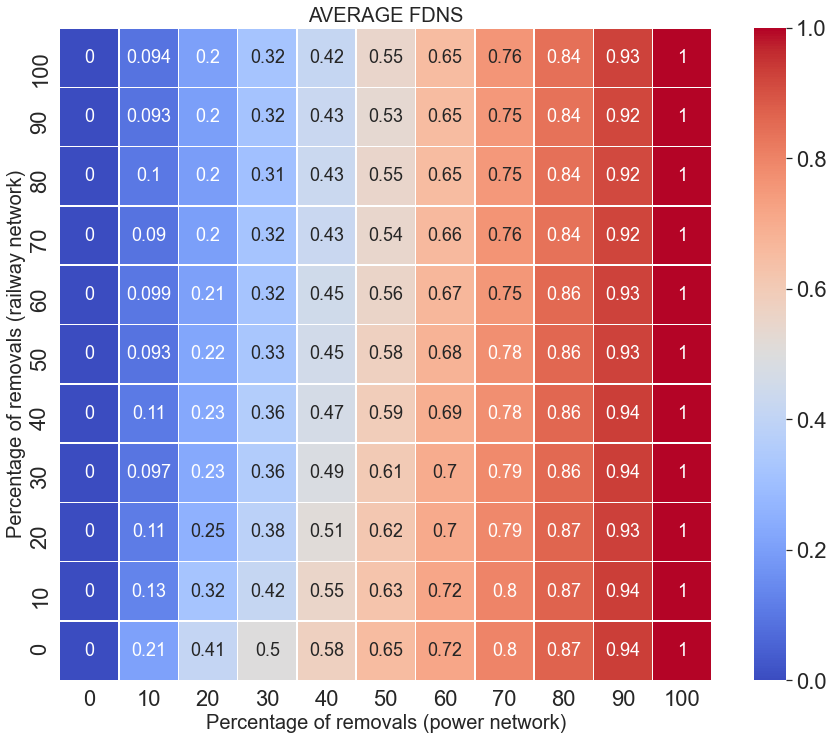
\includegraphics[width=8cm]{images/vuln_power_ccf_100.png}}
	\caption{Vulnerability of the power network with simultaneous random removals in both the networks and $T_{r \leftarrow p}^{P_L}=1.0$. Results of 500 experiments for fraction of removals. Confidence intervals are not shown.}
	\label{vuln_power_ccf_100}
\end{figure}






\section{Discussion}
\subsection{Scenario 1}

	A first conclusion that can be drawn from the analysis is that failures in the power network can have a considerable negative impact on the railway network, as it is clearly visible in the vulnerability analysis of Figures \ref{vuln_power_to_rail},\ref{regions_tp100}, \ref{regions_tp50} and \ref{regions_tp0}. However, it is essential to examine the assumptions that we made on the interdependencies, as they can strongly affect the results.
	
	In this work, we assume that the binary state (functional/failed) of each station depends on the power received by its connected load in the power network and a predefined threshold $T_{r \leftarrow p}^{P_L}$. As it is clearly visible in Figure \ref{vuln_power_to_rail}, the lower is the threshold and the lower is the level of disruption (the area under the curve). It is thus important to evaluate as realistically as possible the assumption on $T_{r \leftarrow p}^{P_L}$, in order to estimate correctly the global vulnerability of the railway network due to failures of the electricity supply. The assumption on $T_{r \leftarrow p}^{P_L}$ can reflect realistic situation where provisions for mitigate lack of electricity are present in the railway network (for example, emergency power devices or diesel-fuelled rolling stocks), as well as the priority policy of the railway network in terms of electricity supply over the other consumers. In this work, we assume an homogeneous $T_{r \leftarrow p}^{P_L}$ along the railway stations, but an heterogeneous distribution according to single elements specifications might better reflect a realistic scenario.

	
	The initial assumption on $T_{r \leftarrow p}^{P_L}$ affects not only the magnitude of disruption, but also the failure modes discussed in the previous section, as visible in Figure \ref{perc_fail_power_to_rail}. The magnitude of impact due to the different failure modes on the railway network in the power network depends on the threshold $T_{r \leftarrow p}^{P_L}$ and the specific percentage of removals, which is a direct representation of the magnitude of the external strain. It is then important to understand how the difference in results might indicate different system behaviours.
	
	High percentages of failures due to direct removals (failure mode 1) are an indicator of geographically localized failures in the railway network due to the intrinsic nature of the interdependencies (closest electrical bus). In fact, given a disruptive event in the power network, a potential impact on the railway network is likely to be restricted to the same area of the disruptive event if failure mode 1 is predominant.
	
	On the contrary, with high fractions due to cascading failures (failure mode 2), due to the possible \say{long-range} features of the phenomenon, failures propagation in areas not originally interested by the disruptive event are more likely to happen. This effect is shown in the analysis of scenario 2, and it depends on the specific features of the area subjected to the disruptive event, as clearly visible in Figures \ref{regions_tp100}, \ref{regions_tp50} and \ref{regions_tp0}. 
	
	The fractions due to disconnection (failure mode 3), are negligible or generally much lower than the first two, and they are strongly related to the topological properties of the railway network itself. However, it has the potential of causing "long-range" disruption in the railway network.
	
	Generally, we can conclude that this analysis shows the importance of the initial assumption of $T_{r \leftarrow p}^{P_L}$, as it can strongly affect the magnitude of the negative consequences of power network failures on the railway network. In addition, different values of $T_{r \leftarrow p}^{P_L}$ lead also to different failure modes contributions. In a critical infrastructures protection perspective, it is essential to understand if, given a specific strain, a failure propagation from the power network to the railway network is more probable to be geographically bounded ("direct removal" failure mode) or it can likely lead to "long-range" failure propagations ("cascading" or "disconnection" failure mode).
	
\subsection{Scenario 2}
	
	The disrupting effect of spatially-localized removals strongly depends on the features of the area under attack (location, number of elements and connections, power generation, power demand, topological location, etc.). In this section, we refer only to Figure \ref{regions_tp100} ($T_{r \leftarrow p}^{P_L}=1.0$), as the greater magnitude of disruption makes the following analysis more intuitive and understandable. We identify three main effects which contribute to the increasing or decreasing disruption trends:
	\begin{itemize}
	    \item Decrease (increase) of power generation-to-demand ratio usually has a negative (positive) effect, that increases (decreases) the magnitude of disruption,
	    \item flow redistribution usually might cause some overloads, increasing the magnitude of disruption,
	    \item islanding (the power network is divided in different independent sub-islands) has usually a positive effect, decreasing the level of disruption.
	\end{itemize}
	Each effect contributes differently, and the total trend depends on their combined effects.
	
	The decrease of power generation-to-demand ratio implies a reduction of the margin between available power generation capacity and power demand, therefore increasing the likelihood of some load shedding and disruption from the power network to the railway network. For example, this effect is predominant when elements from region 1 are removed. In fact, region 1 has an excess of power production, as it shown in Table \ref{regions_features}, and removals in this area likely lead to a reduction of the of power generation-to-demand ratio. Moreover, given its peripheral topological position, this effect is not counterbalanced by other ones, and the total number of failed stations increases monotonically with the fraction of removals.
	
	As a consequence of failures and removals of elements, the power flow can be redistributed along alternative paths from generators to loads. This flow reconfiguration can contribute to failure propagation when some additional lines are overloaded and failed. This effect is predominant, for example, for the increasing disruption in region 2 and 3 with percentages of removals lower than 60\% in region 4 (see Figure \ref{regions_tp100}).
	
	For higher percentages of removals in region 4, the number of failed stations in region 2 and 3 (and in total) decreases. This behaviour is caused by the islanding effect. Failures in region 4 causes failures in region 5 and 6 (in the plot, the line for region 5 and 6 are coincident), and the power network is likely to be reduced to one sub-island, formed by region 1,2 and 3. This decreases the amount of power which, from the upper regions (1,2 and 3), must flows to fulfill the power demands of the lower regions, reducing the magnitude of disruption in the upper part of the network due to flow redistribution, as it is discernible from the descending trends of regions 2 and 3.
	
	Generally, we can conclude that, in case of spatially-localized removals in the power network, the impact on the railway network strongly depends on the features of the region of the power network subjected to the initiating event. Spatially-localized removals are used to represent damages of extreme weather events, like storms and floods, which are, in some measures, forecastable in terms of location and magnitude. In a critical infrastructures protection perspective, it is thus essential to acknowledge that, given a forecastable disruptive event in the power network, a spatially-localized vulnerability analysis is a powerful tool to anticipate possible negative consequences on the railway network, in terms of magnitude and location, which can help to optimize preventive measures and resource allocation.

%	\begin{table}[h]
%	\centering
%	\caption{Regional power production and demand (total and connected to railway network).}
%	\begin{tabular}[t]{lccc}
		%\hline
		%\textbf{Region}& \textbf{Generation [MW]} & \textbf{Load$_{\mathbf{tot}}$ [MW]} & %\textbf{Load$_{\mathbf{rail}}$ [MW]}\\
%		\hline
%		1 & 2174.96 & 981 & 0.0  \\
%		2 & 8942.97 & 7094.5 & 4371.0 \\
%		3 & 14525.73 &  15068.0 &  11708.0 \\
%		4 & 14008.20 & 10087.36 & 3614.0  \\
%		5 & 7977.33 & 7311.0 & 7311.0\\
%		6 & 9662.03 & 15784.0 & 9734.0 \\
%		\hline
%	\end{tabular}
%	\label{regions_features}
%\end{table}%

	\begin{table}[h]
	\centering
	\caption{Regional power production and demand.}
	\begin{tabular}[t]{ccc}
		\hline
		\textbf{Region}& \textbf{Generation [MW]} & \textbf{Demand [MW]}\\
		\hline
		1 & 2174.96 & 981   \\
		2 & 8942.97 & 7094.5  \\
		3 & 14525.73 &  15068.0  \\
		4 & 14008.20 & 10087.36  \\
		5 & 7977.33 & 7311.0 \\
		6 & 9662.03 & 15784.0 \\
		\hline
	\end{tabular}
	\label{regions_features}
\end{table}%
\subsection{Scenario 3}
Random removals of different fractions of elements in both the networks are used to simulate disruptive events, like extreme natural hazards, which might cause damages in both railway and power networks. Intuitively, the magnitude of disruption in the railway network is directly proportional to the fraction of removals in both the networks. In fact, failures in the power network can cause load shedding and additional disruption in the railway network. This behaviour is intuitive and in line with the previous analysis, where only initial removals in the power network were taken into account. As it is clearly shown in Figure \ref{vuln_rail_ccf_100}, where the loss of accessibility is directly proportional to $f_r$ and $f_p$.

On the contrary, the average FDNS is directly proportional to the fraction of removals in the power network, but inversely proportional to the fraction of removals in the railway network. In fact, when a station fails, the corresponding load demand in the power network is reduced. As a consequence, the ratio between power generation capacity and power demand increases, leading to a more robust configuration of the power network. This behaviour is clearly visible from Figure \ref{vuln_power_ccf_100}, where, for a fixed fraction of removals in the power network $f_p$, the average normalized FDNS decreases as the fraction of removals in the railway network $f_r$ increases. It must be highlighted that, as it was already mentioned in section 3, this behaviour is emphasized in terms of magnitude, but not modified in terms of  overall trend, by the assumption that loads connected to the railway network represent exclusively the power consumption of the latter. Despite being not totally realistic, this assumption is suitable for the purpose of this study, as it allows to accentuate and better characterize the aforementioned behaviour. This trend can be characterized as a clear evidence of antifragility in interdependent railway and power networks, where antifragility is defined as the tendency of a system to improve its performance after the exposure to strains and/or failures \cite{fang2017emergence}. We can generalize this behaviour with the following statement: \textit{given a system of interdependent networks, sharing a unidirectional interdependency of the type supplier-consumer, stressors, strains or disruptions in the consumer network can decrease the vulnerability of the supplier network, as the margin between supply generation capacity and total demand increases.}


In conclusion, simultaneous removals of elements in both the networks can represent realistic scenarios (extreme weather events, intentional attacks), which is important to assess considering the interdependencies between the networks. In a protection perspective, this integrated analysis allows to analyze the vulnerability of railway network without underestimations and the vulnerability of power networks without overestimations. In the context of interdependent systems, this kind of integrated analysis is essential for an adequate integrated planning of preventive measures and resource allocation.

\section{Conclusion}
In this work, we have proposed a modeling framework for interdependent railway-power networks, including cascading failures within and between networks. The results of the vulnerability analysis show a considerable disruptive potential of the power network on the railway network, both in the cases of random and spatially-localized removals. In addition, we performed a vulnerability analysis with simultaneous removals in both the networks, highlighting the importance of a correct estimation of a the network vulnerability accounting for the interdependency effects between networks. We have also identified and generalize a behaviour of interdependent supplier-consumer networks which can be interpreted as an evidence of antifragility features. Further developments of this work will include a more precise estimation of the effect of lack of power on the railway network and the introduction of the telecommunications network for vulnerability analysis of interdependent cyber-physical railway and power networks.

	\begin{figure*}[h]
	\centering
	\rotatebox{270}{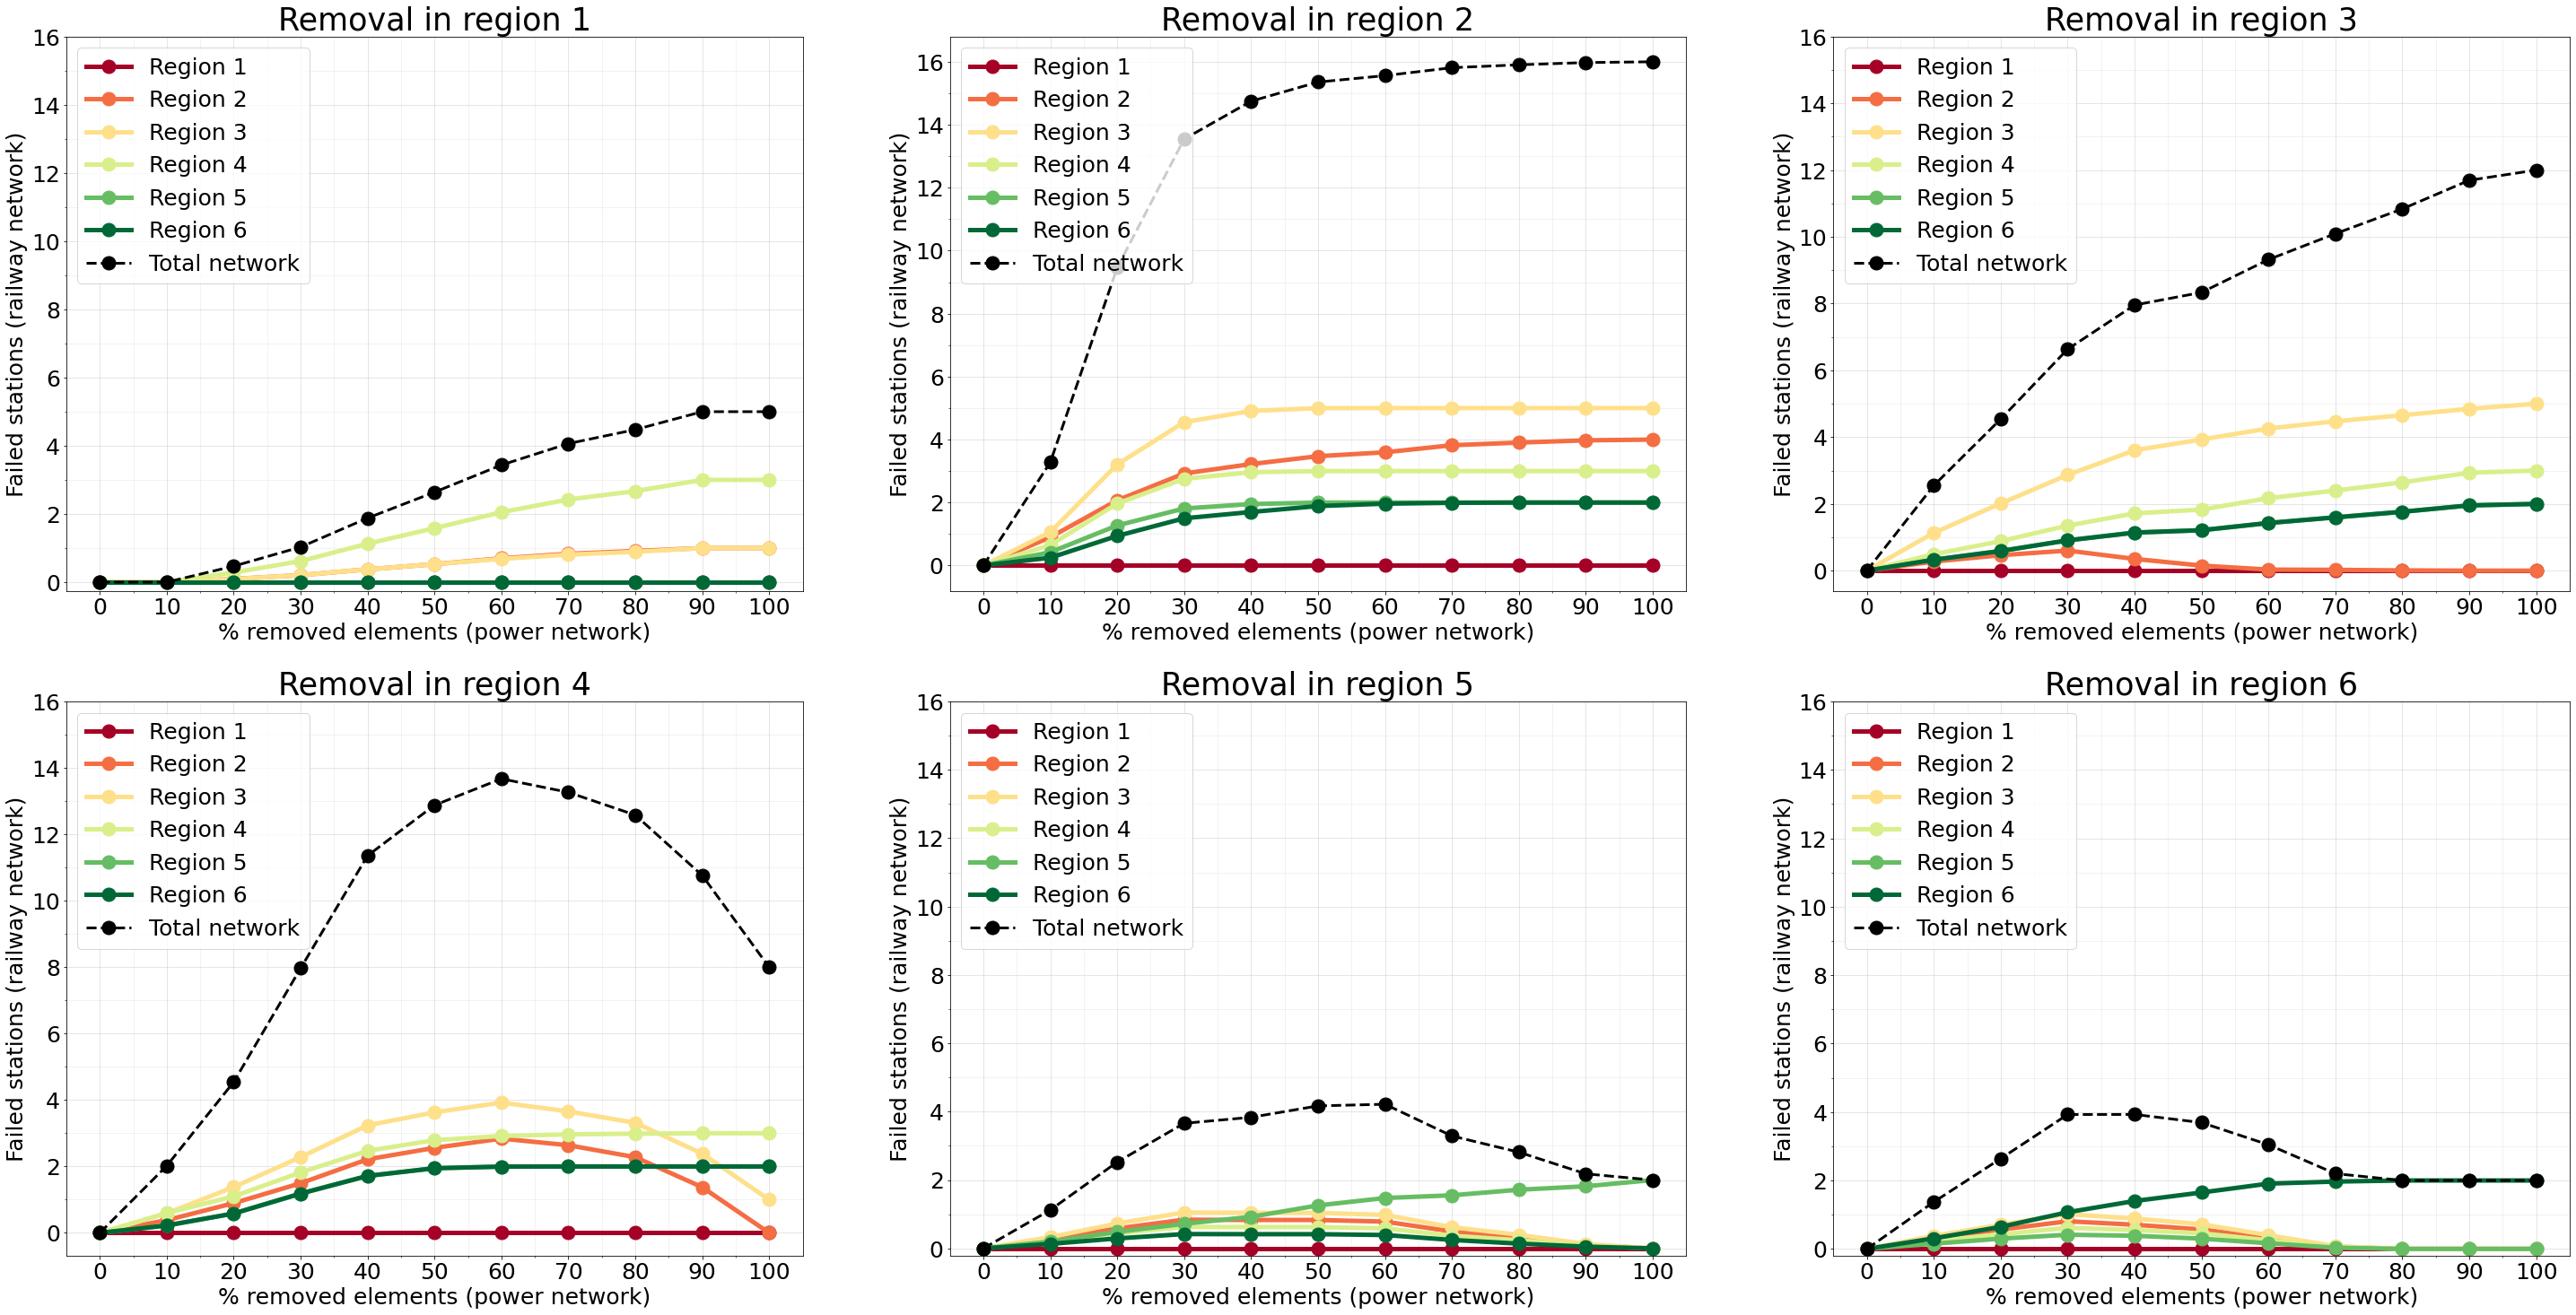
\includegraphics[width=18cm]{images/vuln_regions_t100.png}}
	\caption{Average number of railway stations lost in each region for removal of different fraction of elements in the power network in each region with $T_{r \leftarrow p}^{P_L}=1.0$. Results of 500 experiments for fraction of removals. Confidence intervals are not shown for a clear visualization.}
	\label{regions_tp100}
\end{figure*}

	\begin{figure*}[h]
	\centering
	\rotatebox{270}{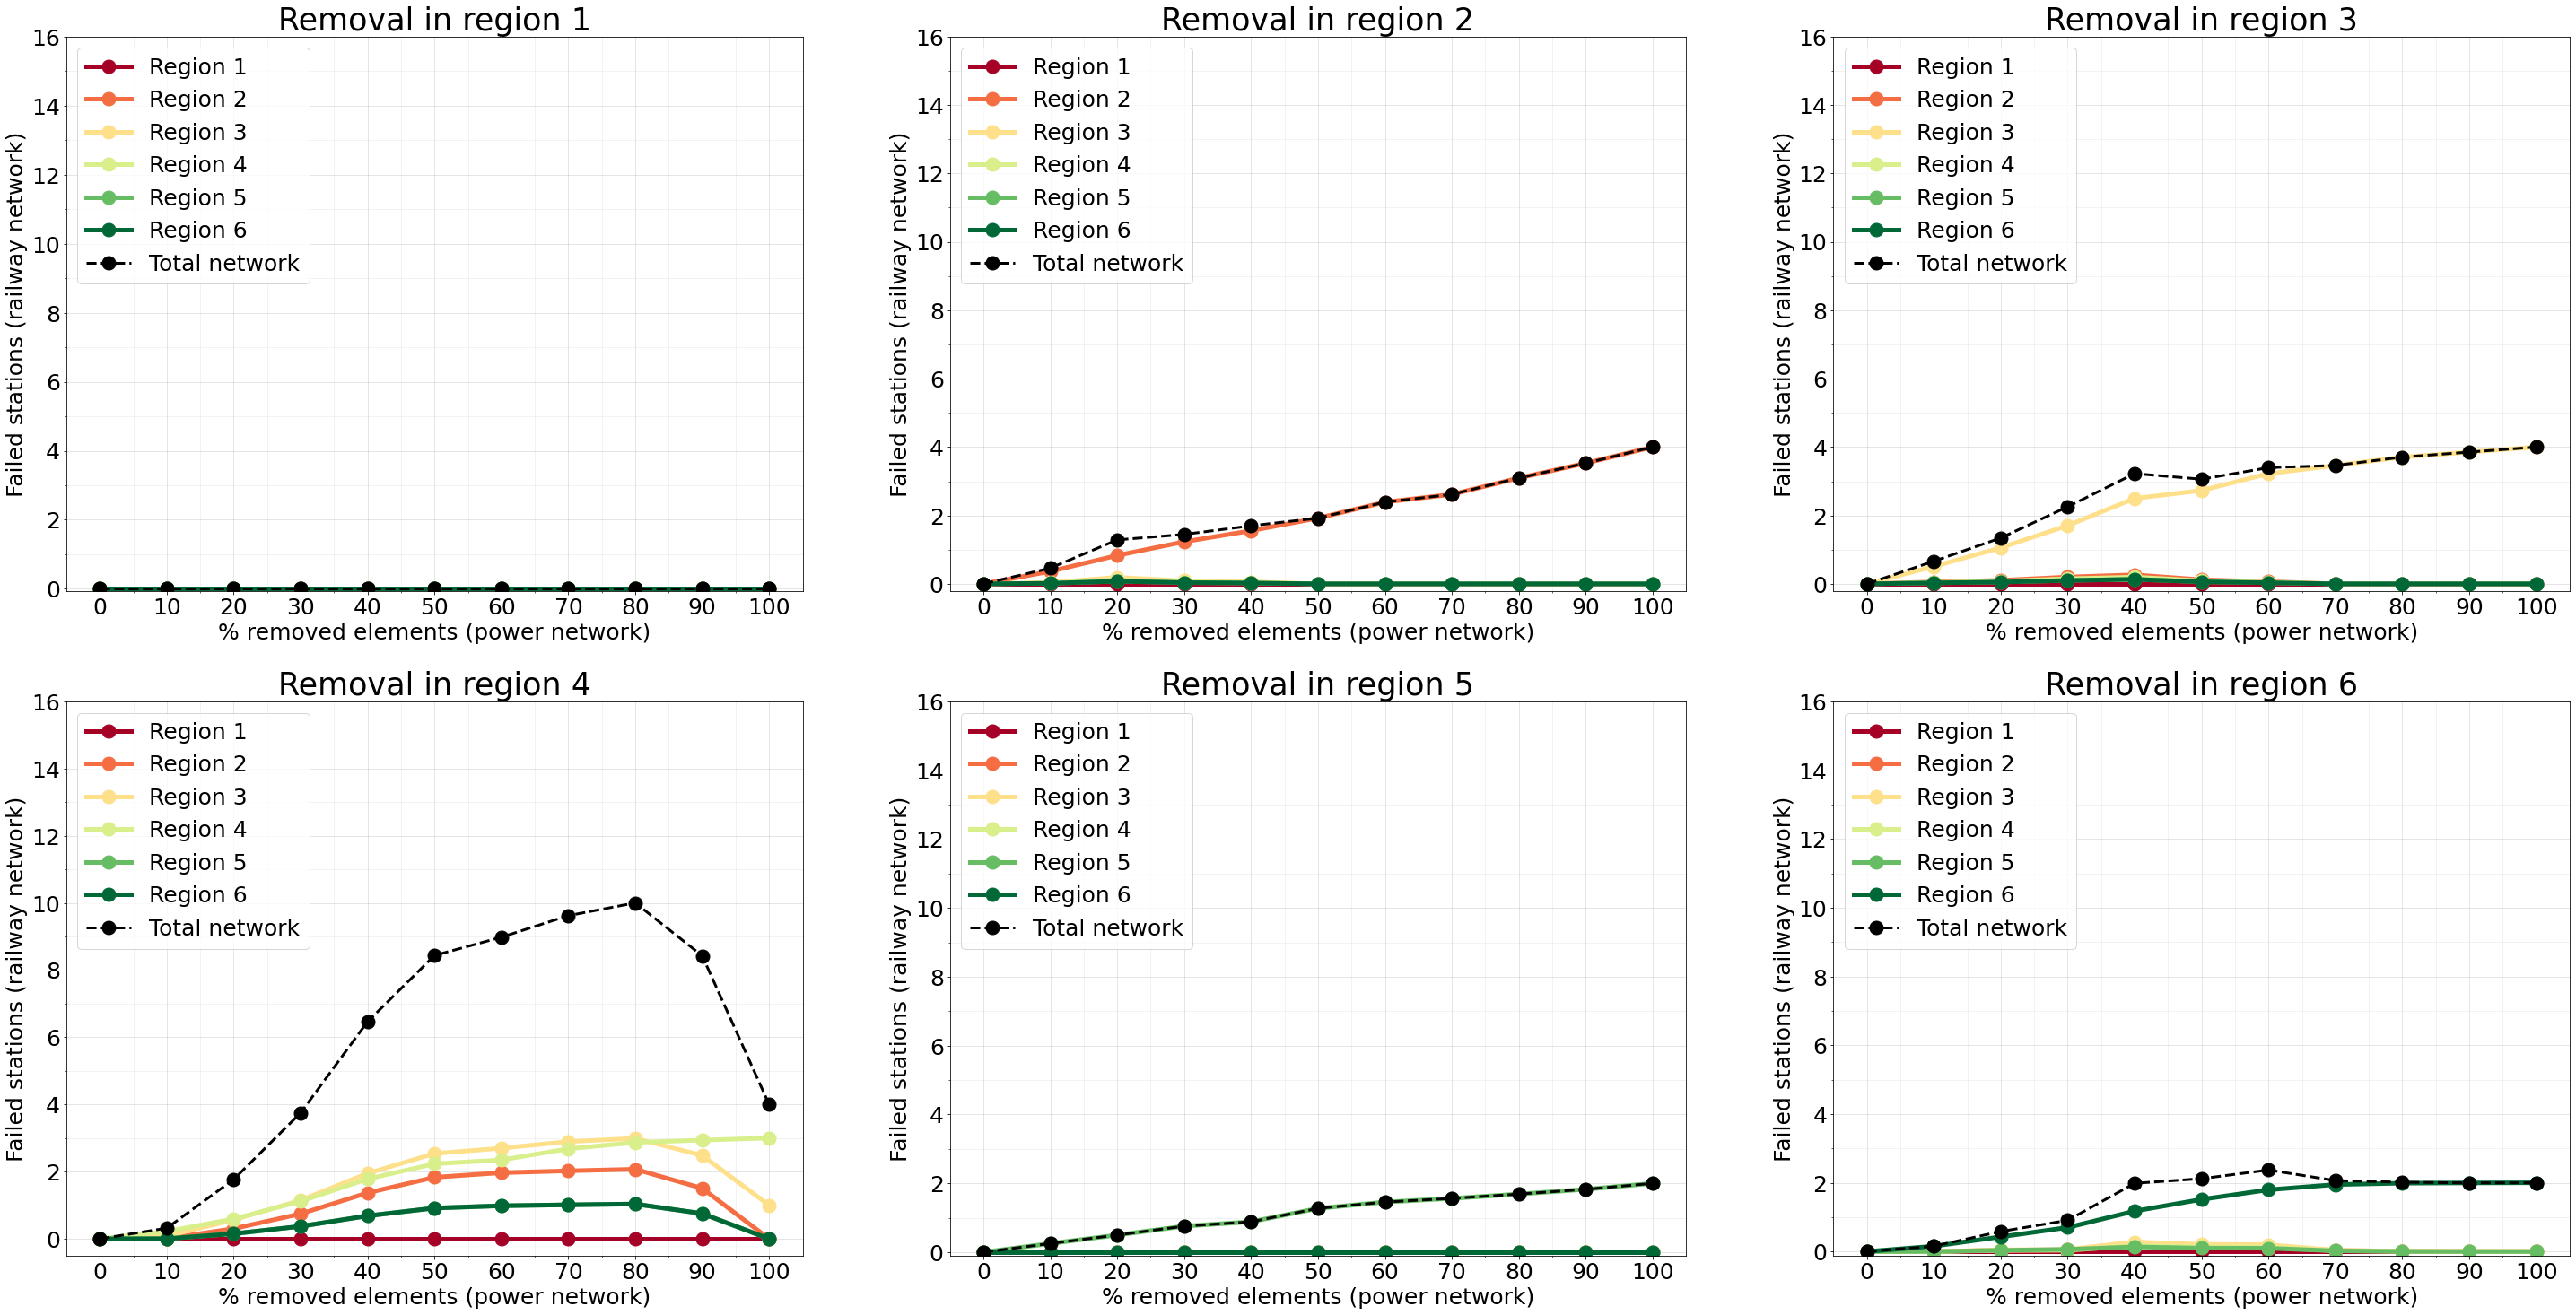
\includegraphics[width=18cm]{images/vuln_regions_t50.png}}
	\caption{Average number of railway stations lost in each region for removal of different fraction of elements in the power network in each region with $T_{r \leftarrow p}^{P_L}=0.5$. Results of 500 experiments for fraction of removals. Confidence intervals are not shown for a clear visualization.}
	\label{regions_tp50}
\end{figure*}



	\begin{figure*}[h]
	\centering
	\rotatebox{270}{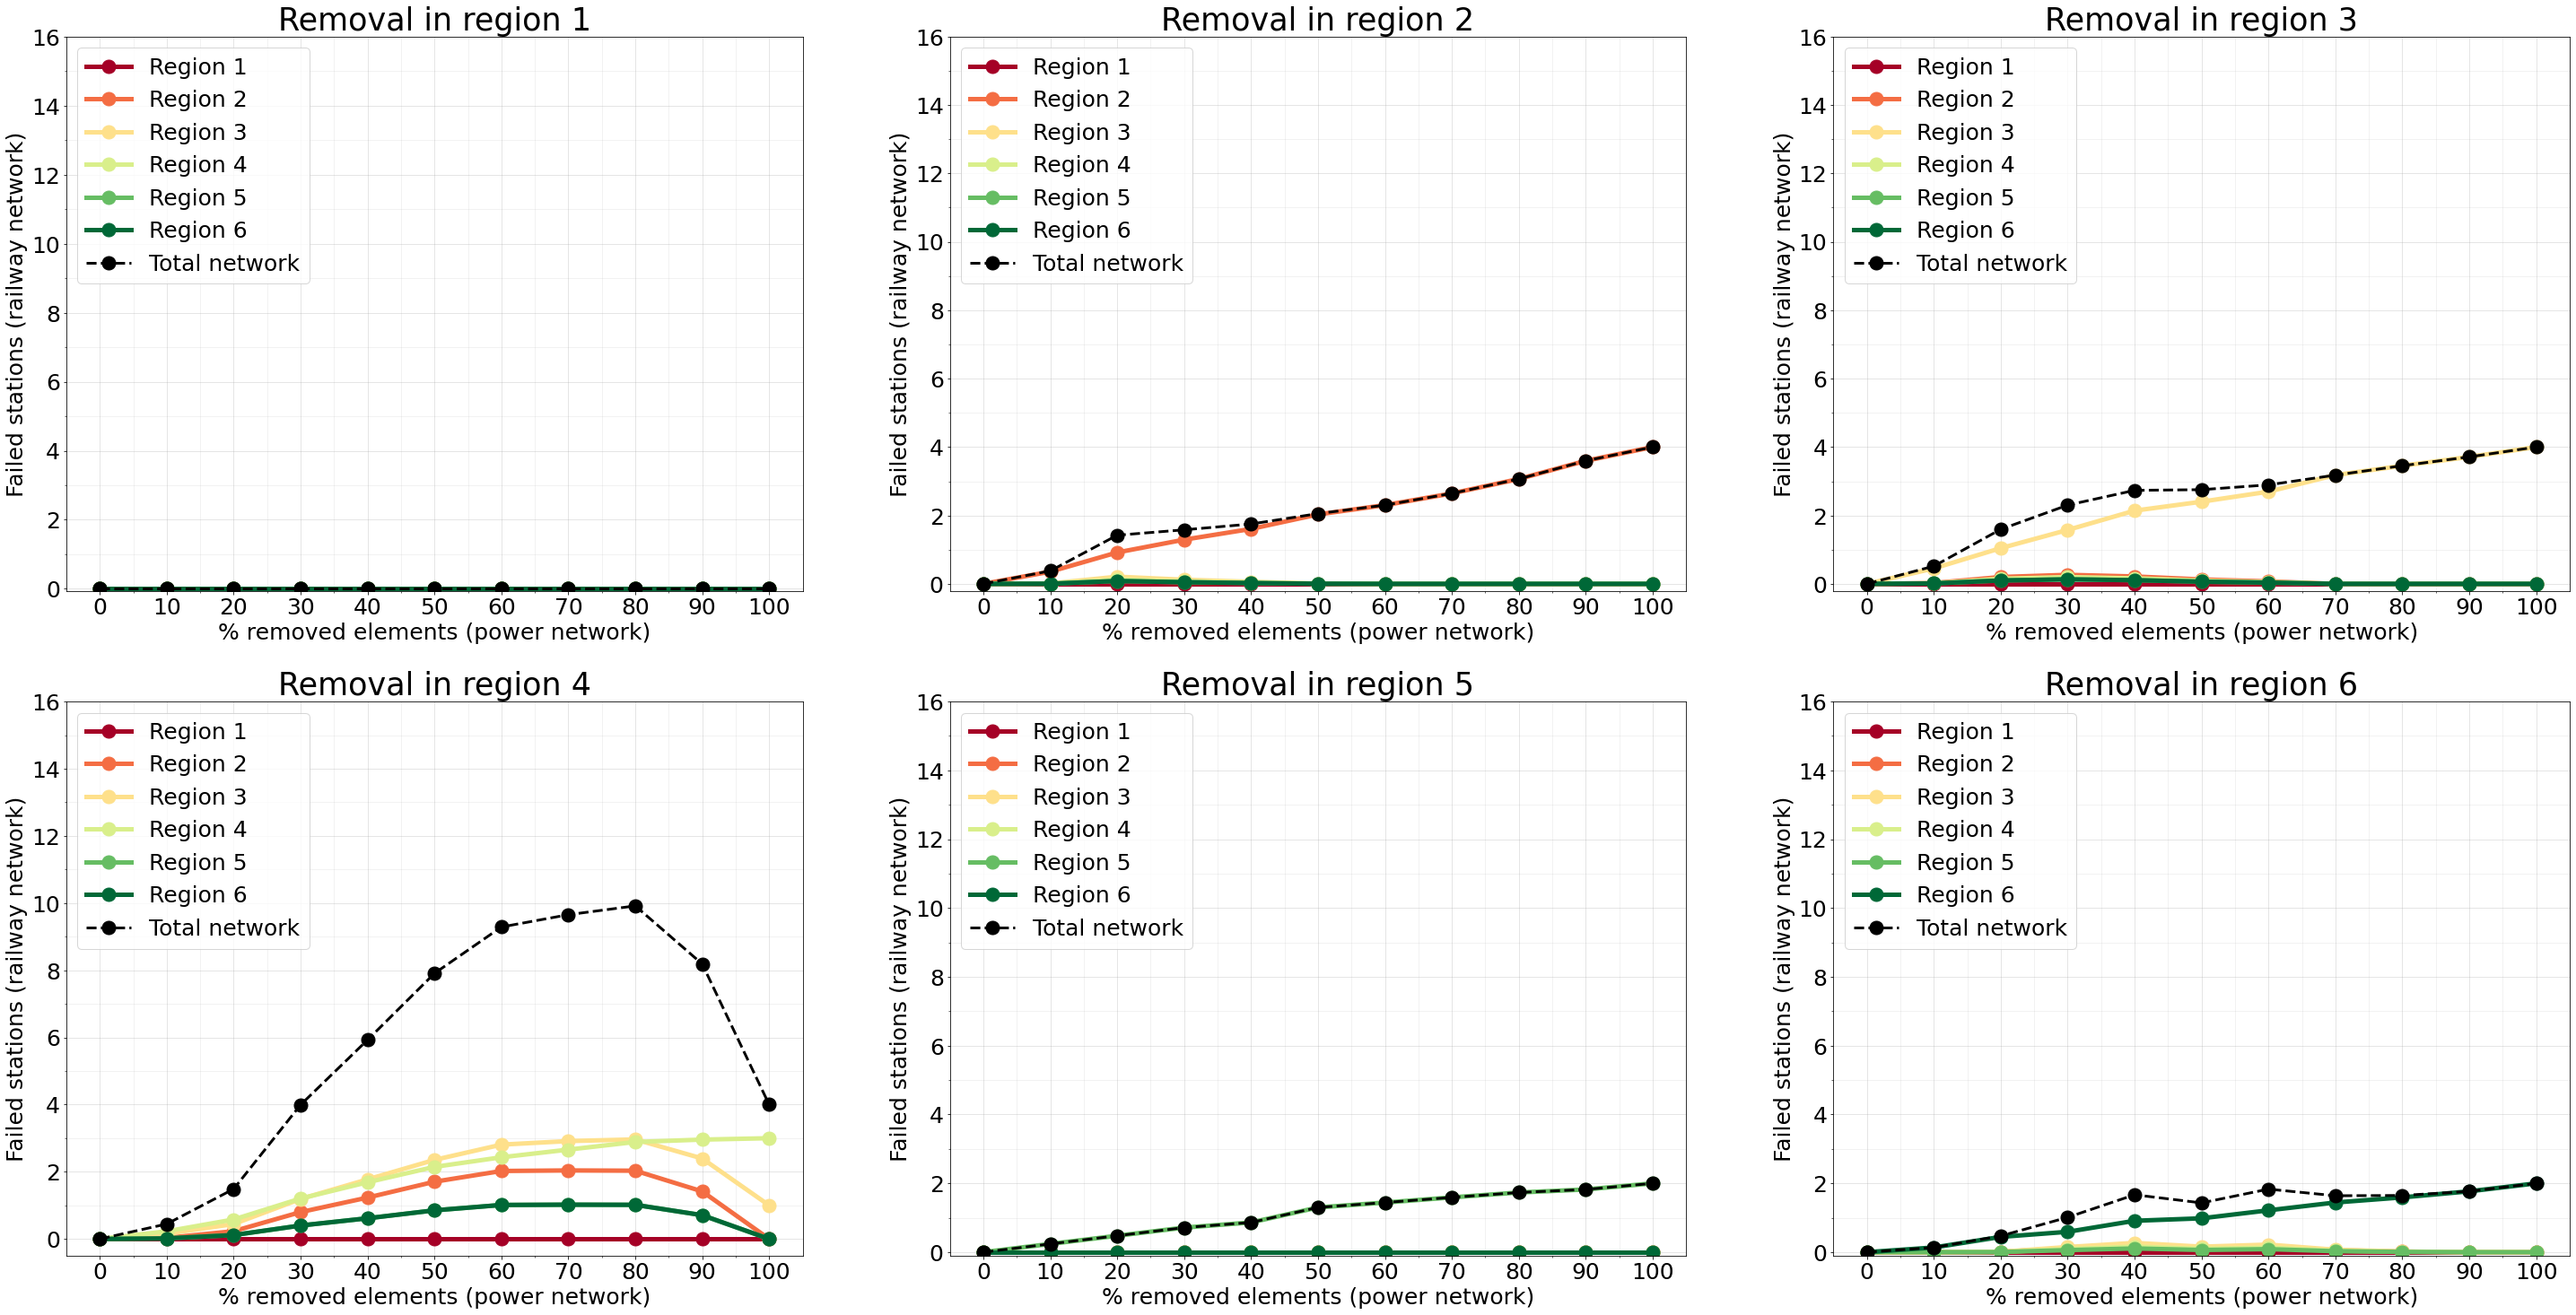
\includegraphics[width=18cm]{images/vuln_regions_t0.png}}
	\caption{Average number of railway stations lost in each region for removal of different fraction of elements in the power network in each region with $T_{r \leftarrow p}^{P_L}=0.0$. Results of 500 experiments for fraction of removals. Confidence intervals are not shown for a clear visualization.}
	\label{regions_tp0}
\end{figure*}

\appendix
\section{DC power flow model}
Active and reactive power injections at bus $i$ are defined, in the AC power flow model, respectively by Equations \ref{active} and \ref{reactive}:
\begin{equation}
    P_i = V_i\sum_{j=1}^N V_j(G_{ij}\,\text{cos}\,\delta_{ij}+B_{ij}\,\text{sin}\,\delta_{ij})
    \label{active}
\end{equation}
\begin{equation}
    Q_i = V_i\sum_{j=1}^N V_j(G_{ij}\,\text{sin}\,\delta_{ij}-B_{ij}\,\text{cos}\,\delta_{ij})
    \label{reactive}
\end{equation}
where $P_i$ and $Q_i$ are the active and reactive power injections at bus $i$, $V_i$ the voltage magnitude, $\delta_{ij}=\delta_i-\delta_j$ the voltage angle difference between buses $i$ and $j$, $G_{ij}$ and $B_{ij}$ respectively the real and imaginary part of admittance matrix elements and $N$ the number of buses. This formulation is non-linear, and it is usually solved by applying Gauss-Seidel or Newton-Raphson method, resulting in computationally expensive simulations. The DC power flow model represents an approximation of the aforementioned AC power flow model. It consists in a linearization of the power flow equations, and it is based on three main assumptions:
\begin{enumerate}
    \item The electrical resistance of each line $i$ is negligible.
    \begin{equation}
        R_{l,i} \approx 0
    \end{equation}
    \item The voltage magnitude at each bus $i$ are equal to 1.
    \begin{equation}
        |V_{i}| = 1
    \end{equation}    
    \item The voltage angle difference between two buses $i$ and $j$, connected by the same line, is small. The trigonometric terms can thus be linearized:
    \begin{equation}
        \text{sin}\,\delta_{ij} \approx \delta_i - \delta_j
    \end{equation}
    \begin{equation}
        \text{cos}\,\delta_{ij} \approx 1.
    \end{equation}
\end{enumerate}
Given these assumptions, the active power injection at bus $i$ and the power flow in line $k$ between bus $i$ and $j$ are expressed in Equations \ref{dc_active} and \ref{dc_flow}:
    \begin{equation}
        P_{i} = \sum_{j=1}^N B_{ij}(\delta_i - \delta_j)
    \label{dc_active}
    \end{equation}
    \begin{equation}
        F_{l,k} = \frac{\delta_i - \delta_j}{X_{l,k}}
        \label{dc_flow}
    \end{equation}
where $X_{l,k}$ is the reactance of line $k$. The DC power flow model can be expressed also in matrix form as following:
\begin{equation}
    \boldsymbol{\Bar{\delta}} = \mathbf{B_N}^{-1}\cdot \mathbf{P_N}
\end{equation}
\begin{equation}
    \mathbf{F_l} = \mathbf{B_d}\cdot\mathbf{A}\cdot \Bar{\delta}
\end{equation}
where $\mathbf{B_N}$ is the admittance matrix with resistance equal to 0, $\boldsymbol{\Bar{\delta}}$ is the bus voltage angle vector, $B_d$ is the diagonal line susceptance matrix and $A$ is the line incidence matrix. For more details on derivation and application of the DC power flow model, the reader is referred to specialized literature \cite{grainger2003power, van2014dc, glover2012power, glover2012power, li2014risk}. 
%\appendices




% references section

% can use a bibliography generated by BibTeX as a .bbl file
% BibTeX documentation can be easily obtained at:
% http://mirror.ctan.org/biblio/bibtex/contrib/doc/
% The IEEEtran BibTeX style support page is at:
% http://www.michaelshell.org/tex/ieeetran/bibtex/
%\bibliographystyle{IEEEtran}
% argument is your BibTeX string definitions and bibliography database(s)
%\bibliography{IEEEabrv,../bib/paper}
%
% <OR> manually copy in the resultant .bbl file
% set second argument of \begin to the number of references
% (used to reserve space for the reference number labels box)

%use following command to generate the list of cited references

\printbibliography







\end{document}


